\documentclass[oneside]{book}
\usepackage[UKenglish]{babel}
\usepackage{graphicx}
\usepackage{natbib}
\usepackage[colorlinks]{hyperref}
\usepackage[dvipsnames]{xcolor}
\usepackage{ amssymb, dsfont }
\usepackage{tikz}
\usepackage{dsfont}

\hypersetup{
  linkcolor  = Magenta,
  citecolor  = Aquamarine,
  urlcolor   = Periwinkle,
  linktoc    = page
}
\usepackage{algorithm}
\usepackage[noend]{algpseudocode}
\usepackage{amsmath,amssymb,bm}

\usepackage{enumitem}
\usepackage{subcaption}
\usepackage{wrapfig}
\usepackage{minted}  % Code embedding in document
\usepackage[none]{hyphenat}

\usepackage{mathtools}
\usepackage{verbatim}

\makeatletter
\newcommand\RedeclareMathOperator{%
  \@ifstar{\def\rmo@s{m}\rmo@redeclare}{\def\rmo@s{o}\rmo@redeclare}%
}
% this is taken from \renew@command
\newcommand\rmo@redeclare[2]{%
  \begingroup \escapechar\m@ne\xdef\@gtempa{{\string#1}}\endgroup
  \expandafter\@ifundefined\@gtempa
     {\@latex@error{\noexpand#1undefined}\@ehc}%
     \relax
  \expandafter\rmo@declmathop\rmo@s{#1}{#2}}
% This is just \@declmathop without \@ifdefinable
\newcommand\rmo@declmathop[3]{%
  \DeclareRobustCommand{#2}{\qopname\newmcodes@#1{#3}}%
}
\@onlypreamble\RedeclareMathOperator
\makeatother

\DeclareMathOperator{\E}{\mathbb{E}}
\DeclareMathOperator{\V}{\mathbb{V}}
\RedeclareMathOperator{\Pr}{\mathbb{P}}
\newcommand{\matr}[1]{\bm{#1}}     % ISO complying version
\newcommand{\vect}[1]{\bm{#1}}     % ISO complying version

\DeclarePairedDelimiter\ceil{\lceil}{\rceil}
\DeclarePairedDelimiter\floor{\lfloor}{\rfloor}

\DeclareMathOperator*{\argmax}{arg\,max}  % in your preamble
\DeclareMathOperator*{\argmin}{arg\,min}  % in your preamble 

\usepackage[nameinlink,noabbrev]{cleveref}
\newcommand*{\fullref}[1]{\hyperref[{#1}]{\Cref*{#1} -- \nameref*{#1}}}

\newcommand{\norm}[1]{\left\lVert#1\right\rVert}


\usepackage[T1]{fontenc}

\usepackage{adjustbox} % Used to constrain images to a maximum size 
\usepackage{xcolor} % Allow colors to be defined
\usepackage{geometry} % Used to adjust the document margins
\usepackage{amsmath} % Equations
\usepackage{amssymb} % Equations
\usepackage{textcomp} % defines textquotesingle
% Hack from http://tex.stackexchange.com/a/47451/13684:
\AtBeginDocument{%
\def\PYZsq{\textquotesingle}% Upright quotes in Pygmentized code
}
\usepackage{upquote} % Upright quotes for verbatim code
\usepackage{eurosym} % defines \euro
\usepackage[mathletters]{ucs} % Extended unicode (utf-8) support
\usepackage[utf8x]{inputenc} % Allow utf-8 characters in the tex document
\usepackage{fancyvrb} % verbatim replacement that allows latex
\usepackage{grffile} % extends the file name processing of package graphics 
% to support a larger range 
% The hyperref package gives us a pdf with properly built
% internal navigation ('pdf bookmarks' for the table of contents,
% internal cross-reference links, web links for URLs, etc.)
\usepackage{hyperref}
\usepackage{longtable} % longtable support required by pandoc >1.10
\usepackage{booktabs}  % table support for pandoc > 1.12.2
\usepackage[normalem]{ulem} % ulem is needed to support strikethroughs (\sout)
% normalem makes italics be italics, not underlines

% ANSI colors
\definecolor{ansi-black}{HTML}{3E424D}
\definecolor{ansi-black-intense}{HTML}{282C36}
\definecolor{ansi-red}{HTML}{E75C58}
\definecolor{ansi-red-intense}{HTML}{B22B31}
\definecolor{ansi-green}{HTML}{00A250}
\definecolor{ansi-green-intense}{HTML}{007427}
\definecolor{ansi-yellow}{HTML}{DDB62B}
\definecolor{ansi-yellow-intense}{HTML}{B27D12}
\definecolor{ansi-blue}{HTML}{208FFB}
\definecolor{ansi-blue-intense}{HTML}{0065CA}
\definecolor{ansi-magenta}{HTML}{D160C4}
\definecolor{ansi-magenta-intense}{HTML}{A03196}
\definecolor{ansi-cyan}{HTML}{60C6C8}
\definecolor{ansi-cyan-intense}{HTML}{258F8F}
\definecolor{ansi-white}{HTML}{C5C1B4}
\definecolor{ansi-white-intense}{HTML}{A1A6B2}

% commands and environments needed by pandoc snippets
% extracted from the output of `pandoc -s`
\providecommand{\tightlist}{%
\setlength{\itemsep}{0pt}\setlength{\parskip}{0pt}}
\DefineVerbatimEnvironment{Highlighting}{Verbatim}{commandchars=\\\{\}}
% Add ',fontsize=\small' for more characters per line
\newenvironment{Shaded}{}{}
\newcommand{\KeywordTok}[1]{\textcolor[rgb]{0.00,0.44,0.13}{\textbf{{#1}}}}
\newcommand{\DataTypeTok}[1]{\textcolor[rgb]{0.56,0.13,0.00}{{#1}}}
\newcommand{\DecValTok}[1]{\textcolor[rgb]{0.25,0.63,0.44}{{#1}}}
\newcommand{\BaseNTok}[1]{\textcolor[rgb]{0.25,0.63,0.44}{{#1}}}
\newcommand{\FloatTok}[1]{\textcolor[rgb]{0.25,0.63,0.44}{{#1}}}
\newcommand{\CharTok}[1]{\textcolor[rgb]{0.25,0.44,0.63}{{#1}}}
\newcommand{\StringTok}[1]{\textcolor[rgb]{0.25,0.44,0.63}{{#1}}}
\newcommand{\CommentTok}[1]{\textcolor[rgb]{0.38,0.63,0.69}{\textit{{#1}}}}
\newcommand{\OtherTok}[1]{\textcolor[rgb]{0.00,0.44,0.13}{{#1}}}
\newcommand{\AlertTok}[1]{\textcolor[rgb]{1.00,0.00,0.00}{\textbf{{#1}}}}
\newcommand{\FunctionTok}[1]{\textcolor[rgb]{0.02,0.16,0.49}{{#1}}}
\newcommand{\RegionMarkerTok}[1]{{#1}}
\newcommand{\ErrorTok}[1]{\textcolor[rgb]{1.00,0.00,0.00}{\textbf{{#1}}}}
\newcommand{\NormalTok}[1]{{#1}}

% Additional commands for more recent versions of Pandoc
\newcommand{\ConstantTok}[1]{\textcolor[rgb]{0.53,0.00,0.00}{{#1}}}
\newcommand{\SpecialCharTok}[1]{\textcolor[rgb]{0.25,0.44,0.63}{{#1}}}
\newcommand{\VerbatimStringTok}[1]{\textcolor[rgb]{0.25,0.44,0.63}{{#1}}}
\newcommand{\SpecialStringTok}[1]{\textcolor[rgb]{0.73,0.40,0.53}{{#1}}}
\newcommand{\ImportTok}[1]{{#1}}
\newcommand{\DocumentationTok}[1]{\textcolor[rgb]{0.73,0.13,0.13}{\textit{{#1}}}}
\newcommand{\AnnotationTok}[1]{\textcolor[rgb]{0.38,0.63,0.69}{\textbf{\textit{{#1}}}}}
\newcommand{\CommentVarTok}[1]{\textcolor[rgb]{0.38,0.63,0.69}{\textbf{\textit{{#1}}}}}
\newcommand{\VariableTok}[1]{\textcolor[rgb]{0.10,0.09,0.49}{{#1}}}
\newcommand{\ControlFlowTok}[1]{\textcolor[rgb]{0.00,0.44,0.13}{\textbf{{#1}}}}
\newcommand{\OperatorTok}[1]{\textcolor[rgb]{0.40,0.40,0.40}{{#1}}}
\newcommand{\BuiltInTok}[1]{{#1}}
\newcommand{\ExtensionTok}[1]{{#1}}
\newcommand{\PreprocessorTok}[1]{\textcolor[rgb]{0.74,0.48,0.00}{{#1}}}
\newcommand{\AttributeTok}[1]{\textcolor[rgb]{0.49,0.56,0.16}{{#1}}}
\newcommand{\InformationTok}[1]{\textcolor[rgb]{0.38,0.63,0.69}{\textbf{\textit{{#1}}}}}
\newcommand{\WarningTok}[1]{\textcolor[rgb]{0.38,0.63,0.69}{\textbf{\textit{{#1}}}}}


% Define a nice break command that doesn't care if a line doesn't already
% exist.
\def\br{\hspace*{\fill} \\* }
% Math Jax compatability definitions
\def\gt{>}
\def\lt{<}
% Document parameters
\title{PyTorch\_nn}




    % Pygments definitions

\makeatletter
\def\PY@reset{\let\PY@it=\relax \let\PY@bf=\relax%
    \let\PY@ul=\relax \let\PY@tc=\relax%
    \let\PY@bc=\relax \let\PY@ff=\relax}
\def\PY@tok#1{\csname PY@tok@#1\endcsname}
\def\PY@toks#1+{\ifx\relax#1\empty\else%
    \PY@tok{#1}\expandafter\PY@toks\fi}
\def\PY@do#1{\PY@bc{\PY@tc{\PY@ul{%
    \PY@it{\PY@bf{\PY@ff{#1}}}}}}}
\def\PY#1#2{\PY@reset\PY@toks#1+\relax+\PY@do{#2}}

\expandafter\def\csname PY@tok@w\endcsname{\def\PY@tc##1{\textcolor[rgb]{0.73,0.73,0.73}{##1}}}
\expandafter\def\csname PY@tok@c\endcsname{\let\PY@it=\textit\def\PY@tc##1{\textcolor[rgb]{0.25,0.50,0.50}{##1}}}
\expandafter\def\csname PY@tok@cp\endcsname{\def\PY@tc##1{\textcolor[rgb]{0.74,0.48,0.00}{##1}}}
\expandafter\def\csname PY@tok@k\endcsname{\let\PY@bf=\textbf\def\PY@tc##1{\textcolor[rgb]{0.00,0.50,0.00}{##1}}}
\expandafter\def\csname PY@tok@kp\endcsname{\def\PY@tc##1{\textcolor[rgb]{0.00,0.50,0.00}{##1}}}
\expandafter\def\csname PY@tok@kt\endcsname{\def\PY@tc##1{\textcolor[rgb]{0.69,0.00,0.25}{##1}}}
\expandafter\def\csname PY@tok@o\endcsname{\def\PY@tc##1{\textcolor[rgb]{0.40,0.40,0.40}{##1}}}
\expandafter\def\csname PY@tok@ow\endcsname{\let\PY@bf=\textbf\def\PY@tc##1{\textcolor[rgb]{0.67,0.13,1.00}{##1}}}
\expandafter\def\csname PY@tok@nb\endcsname{\def\PY@tc##1{\textcolor[rgb]{0.00,0.50,0.00}{##1}}}
\expandafter\def\csname PY@tok@nf\endcsname{\def\PY@tc##1{\textcolor[rgb]{0.00,0.00,1.00}{##1}}}
\expandafter\def\csname PY@tok@nc\endcsname{\let\PY@bf=\textbf\def\PY@tc##1{\textcolor[rgb]{0.00,0.00,1.00}{##1}}}
\expandafter\def\csname PY@tok@nn\endcsname{\let\PY@bf=\textbf\def\PY@tc##1{\textcolor[rgb]{0.00,0.00,1.00}{##1}}}
\expandafter\def\csname PY@tok@ne\endcsname{\let\PY@bf=\textbf\def\PY@tc##1{\textcolor[rgb]{0.82,0.25,0.23}{##1}}}
\expandafter\def\csname PY@tok@nv\endcsname{\def\PY@tc##1{\textcolor[rgb]{0.10,0.09,0.49}{##1}}}
\expandafter\def\csname PY@tok@no\endcsname{\def\PY@tc##1{\textcolor[rgb]{0.53,0.00,0.00}{##1}}}
\expandafter\def\csname PY@tok@nl\endcsname{\def\PY@tc##1{\textcolor[rgb]{0.63,0.63,0.00}{##1}}}
\expandafter\def\csname PY@tok@ni\endcsname{\let\PY@bf=\textbf\def\PY@tc##1{\textcolor[rgb]{0.60,0.60,0.60}{##1}}}
\expandafter\def\csname PY@tok@na\endcsname{\def\PY@tc##1{\textcolor[rgb]{0.49,0.56,0.16}{##1}}}
\expandafter\def\csname PY@tok@nt\endcsname{\let\PY@bf=\textbf\def\PY@tc##1{\textcolor[rgb]{0.00,0.50,0.00}{##1}}}
\expandafter\def\csname PY@tok@nd\endcsname{\def\PY@tc##1{\textcolor[rgb]{0.67,0.13,1.00}{##1}}}
\expandafter\def\csname PY@tok@s\endcsname{\def\PY@tc##1{\textcolor[rgb]{0.73,0.13,0.13}{##1}}}
\expandafter\def\csname PY@tok@sd\endcsname{\let\PY@it=\textit\def\PY@tc##1{\textcolor[rgb]{0.73,0.13,0.13}{##1}}}
\expandafter\def\csname PY@tok@si\endcsname{\let\PY@bf=\textbf\def\PY@tc##1{\textcolor[rgb]{0.73,0.40,0.53}{##1}}}
\expandafter\def\csname PY@tok@se\endcsname{\let\PY@bf=\textbf\def\PY@tc##1{\textcolor[rgb]{0.73,0.40,0.13}{##1}}}
\expandafter\def\csname PY@tok@sr\endcsname{\def\PY@tc##1{\textcolor[rgb]{0.73,0.40,0.53}{##1}}}
\expandafter\def\csname PY@tok@ss\endcsname{\def\PY@tc##1{\textcolor[rgb]{0.10,0.09,0.49}{##1}}}
\expandafter\def\csname PY@tok@sx\endcsname{\def\PY@tc##1{\textcolor[rgb]{0.00,0.50,0.00}{##1}}}
\expandafter\def\csname PY@tok@m\endcsname{\def\PY@tc##1{\textcolor[rgb]{0.40,0.40,0.40}{##1}}}
\expandafter\def\csname PY@tok@gh\endcsname{\let\PY@bf=\textbf\def\PY@tc##1{\textcolor[rgb]{0.00,0.00,0.50}{##1}}}
\expandafter\def\csname PY@tok@gu\endcsname{\let\PY@bf=\textbf\def\PY@tc##1{\textcolor[rgb]{0.50,0.00,0.50}{##1}}}
\expandafter\def\csname PY@tok@gd\endcsname{\def\PY@tc##1{\textcolor[rgb]{0.63,0.00,0.00}{##1}}}
\expandafter\def\csname PY@tok@gi\endcsname{\def\PY@tc##1{\textcolor[rgb]{0.00,0.63,0.00}{##1}}}
\expandafter\def\csname PY@tok@gr\endcsname{\def\PY@tc##1{\textcolor[rgb]{1.00,0.00,0.00}{##1}}}
\expandafter\def\csname PY@tok@ge\endcsname{\let\PY@it=\textit}
\expandafter\def\csname PY@tok@gs\endcsname{\let\PY@bf=\textbf}
\expandafter\def\csname PY@tok@gp\endcsname{\let\PY@bf=\textbf\def\PY@tc##1{\textcolor[rgb]{0.00,0.00,0.50}{##1}}}
\expandafter\def\csname PY@tok@go\endcsname{\def\PY@tc##1{\textcolor[rgb]{0.53,0.53,0.53}{##1}}}
\expandafter\def\csname PY@tok@gt\endcsname{\def\PY@tc##1{\textcolor[rgb]{0.00,0.27,0.87}{##1}}}
\expandafter\def\csname PY@tok@err\endcsname{\def\PY@bc##1{\setlength{\fboxsep}{0pt}\fcolorbox[rgb]{1.00,0.00,0.00}{1,1,1}{\strut ##1}}}
\expandafter\def\csname PY@tok@kc\endcsname{\let\PY@bf=\textbf\def\PY@tc##1{\textcolor[rgb]{0.00,0.50,0.00}{##1}}}
\expandafter\def\csname PY@tok@kd\endcsname{\let\PY@bf=\textbf\def\PY@tc##1{\textcolor[rgb]{0.00,0.50,0.00}{##1}}}
\expandafter\def\csname PY@tok@kn\endcsname{\let\PY@bf=\textbf\def\PY@tc##1{\textcolor[rgb]{0.00,0.50,0.00}{##1}}}
\expandafter\def\csname PY@tok@kr\endcsname{\let\PY@bf=\textbf\def\PY@tc##1{\textcolor[rgb]{0.00,0.50,0.00}{##1}}}
\expandafter\def\csname PY@tok@bp\endcsname{\def\PY@tc##1{\textcolor[rgb]{0.00,0.50,0.00}{##1}}}
\expandafter\def\csname PY@tok@fm\endcsname{\def\PY@tc##1{\textcolor[rgb]{0.00,0.00,1.00}{##1}}}
\expandafter\def\csname PY@tok@vc\endcsname{\def\PY@tc##1{\textcolor[rgb]{0.10,0.09,0.49}{##1}}}
\expandafter\def\csname PY@tok@vg\endcsname{\def\PY@tc##1{\textcolor[rgb]{0.10,0.09,0.49}{##1}}}
\expandafter\def\csname PY@tok@vi\endcsname{\def\PY@tc##1{\textcolor[rgb]{0.10,0.09,0.49}{##1}}}
\expandafter\def\csname PY@tok@vm\endcsname{\def\PY@tc##1{\textcolor[rgb]{0.10,0.09,0.49}{##1}}}
\expandafter\def\csname PY@tok@sa\endcsname{\def\PY@tc##1{\textcolor[rgb]{0.73,0.13,0.13}{##1}}}
\expandafter\def\csname PY@tok@sb\endcsname{\def\PY@tc##1{\textcolor[rgb]{0.73,0.13,0.13}{##1}}}
\expandafter\def\csname PY@tok@sc\endcsname{\def\PY@tc##1{\textcolor[rgb]{0.73,0.13,0.13}{##1}}}
\expandafter\def\csname PY@tok@dl\endcsname{\def\PY@tc##1{\textcolor[rgb]{0.73,0.13,0.13}{##1}}}
\expandafter\def\csname PY@tok@s2\endcsname{\def\PY@tc##1{\textcolor[rgb]{0.73,0.13,0.13}{##1}}}
\expandafter\def\csname PY@tok@sh\endcsname{\def\PY@tc##1{\textcolor[rgb]{0.73,0.13,0.13}{##1}}}
\expandafter\def\csname PY@tok@s1\endcsname{\def\PY@tc##1{\textcolor[rgb]{0.73,0.13,0.13}{##1}}}
\expandafter\def\csname PY@tok@mb\endcsname{\def\PY@tc##1{\textcolor[rgb]{0.40,0.40,0.40}{##1}}}
\expandafter\def\csname PY@tok@mf\endcsname{\def\PY@tc##1{\textcolor[rgb]{0.40,0.40,0.40}{##1}}}
\expandafter\def\csname PY@tok@mh\endcsname{\def\PY@tc##1{\textcolor[rgb]{0.40,0.40,0.40}{##1}}}
\expandafter\def\csname PY@tok@mi\endcsname{\def\PY@tc##1{\textcolor[rgb]{0.40,0.40,0.40}{##1}}}
\expandafter\def\csname PY@tok@il\endcsname{\def\PY@tc##1{\textcolor[rgb]{0.40,0.40,0.40}{##1}}}
\expandafter\def\csname PY@tok@mo\endcsname{\def\PY@tc##1{\textcolor[rgb]{0.40,0.40,0.40}{##1}}}
\expandafter\def\csname PY@tok@ch\endcsname{\let\PY@it=\textit\def\PY@tc##1{\textcolor[rgb]{0.25,0.50,0.50}{##1}}}
\expandafter\def\csname PY@tok@cm\endcsname{\let\PY@it=\textit\def\PY@tc##1{\textcolor[rgb]{0.25,0.50,0.50}{##1}}}
\expandafter\def\csname PY@tok@cpf\endcsname{\let\PY@it=\textit\def\PY@tc##1{\textcolor[rgb]{0.25,0.50,0.50}{##1}}}
\expandafter\def\csname PY@tok@c1\endcsname{\let\PY@it=\textit\def\PY@tc##1{\textcolor[rgb]{0.25,0.50,0.50}{##1}}}
\expandafter\def\csname PY@tok@cs\endcsname{\let\PY@it=\textit\def\PY@tc##1{\textcolor[rgb]{0.25,0.50,0.50}{##1}}}

\def\PYZbs{\char`\\}
\def\PYZus{\char`\_}
\def\PYZob{\char`\{}
\def\PYZcb{\char`\}}
\def\PYZca{\char`\^}
\def\PYZam{\char`\&}
\def\PYZlt{\char`\<}
\def\PYZgt{\char`\>}
\def\PYZsh{\char`\#}
\def\PYZpc{\char`\%}
\def\PYZdl{\char`\$}
\def\PYZhy{\char`\-}
\def\PYZsq{\char`\'}
\def\PYZdq{\char`\"}
\def\PYZti{\char`\~}
% for compatibility with earlier versions
\def\PYZat{@}
\def\PYZlb{[}
\def\PYZrb{]}
\makeatother


% Exact colors from NB
\definecolor{incolor}{rgb}{0.0, 0.0, 0.5}
\definecolor{outcolor}{rgb}{0.545, 0.0, 0.0}

\title{SP19 DL collaborative notes}
\author{
  The students of SP19 Deep Learning\\
  Editor: Alfredo Canziani\\
  NYU
}
\date{\today}

\begin{document}

\maketitle

\chapter*{Preface} \label{chp:preface}

This document aims to be a collection of lecture and laboratory notes, in an attempt to uniform the mathematical notation and gather all resources related to understand and master \emph{deep learning} in one, single location.

These notes are divided in five parts, which will constantly link to each other.
These are \fullref{prt:theory}, where the main topics will be introduced, \fullref{prt:practice}, where an intuition will be built about abstract concepts, \fullref{prt:coding}, where we'll see how to get our hands dirty with actual neural nets, on a computer, \fullref{prt:apps} where we'll encounter real life examples and applications, and \fullref{prt:papers} where short summary of the papers we've discussed will be nicely collected.
\chapter*{Instructions}

There are overall 42 hours of lectures.
For each hour there is a group of people assigned to summarise what happened in class \textbf{in roughly three pages}.
Each group is made of three students: two writers and a reviewer.

\section*{Writing directions}

Split your writing across the five parts of this document according to where it seems fit (see \nameref{chp:preface}).
Be consistent with the notation here specified.
\begin{itemize}[noitemsep,nolistsep]
\item Use \verb|\vect{}| and \verb|\matr{}| to decorate vectors and matrices respectively.
\item Start a new line \textbf{only and every time} you end a sentence with a period `.'; the \LaTeX\ engine will ignore this, but \verb|git| will love you.
\item Leave an empty line to start a new paragraph, and don't use the `\verb|\\|' break line (see \url{tex.stackexchange.com/a/225925/33287}).
\item Add date and group's authors name \textbf{as a comment}, after every \verb|\chapter|, \verb|\section|, and \verb|\subsection|.
\item The transposition symbol is obtained with \verb|^\top|. For example $(AB)^\top = B^\top A^\top$.
\end{itemize}

Feel free to create new chapters, sections, and subsections with corresponding labels \verb|\label{chp:}|, \verb|\label{sct:}|, and \verb|\label{ssc:}|.

\section*{Peer reviewing within groups}

Check for notation consistency, correctness, grammar, figure captioning, usage of \verb|\cref{}| instead of \verb|\ref{}|, \verb|\vect{}|, and \verb|\matr{}| to decorate vectors and matrices respectively, unnecessary use of bullet points or itemisations, missing references and use of links to papers PDF instead, usage of  $\Pr$, $\E$, and $\V$ for probability, expectation, and variance respectively using \verb|\Pr|, \verb|\E|, and \verb|\V|, \verb|\mid| for the conditional vertical bar, missing backslashes for $log, exp, max$ and any badly formatted functions, $\ast$ for convolutions, $\odot$ for element-wise multiplication, usage of \verb|\caption[Short caption]{Full caption}|, use of the correct transposition symbol obtained with \verb|^\top|, just to name a few.

\section*{Taking inspiration}

You can take inspiration from the work done by the students at NYU, who collectively wrote up the lecture notes in \href{https://www.overleaf.com/read/pchjywcxjkxn
}{this document} last year.
For example, you may reuse the following constructs, and others, at your convenience:
\[
\matr{X} = \begin{bmatrix}
    \rule[0.5mm]{0.8cm}{0.1mm} \; \vect{x}^{(1)} \; \rule[0.5mm]{0.8cm}{0.1mm} \\
    \rule[0.5mm]{0.8cm}{0.1mm} \; \vect{x}^{(2)} \; \rule[0.5mm]{0.8cm}{0.1mm} \\
    \vdots \\
    \rule[0.5mm]{0.8cm}{0.1mm} \; \vect{x}^{(m)} \; \rule[0.5mm]{0.8cm}{0.1mm} \\
\end{bmatrix}_{m \times n}
\matr{Y} = \begin{bmatrix}
    \rule[0.5mm]{0.8cm}{0.1mm} \; \vect{y}^{(1)} \; \rule[0.5mm]{0.8cm}{0.1mm} \\
    \rule[0.5mm]{0.8cm}{0.1mm} \; \vect{y}^{(2)} \; \rule[0.5mm]{0.8cm}{0.1mm} \\
    \vdots \\
    \rule[0.5mm]{0.8cm}{0.1mm} \; \vect{y}^{(m)} \; \rule[0.5mm]{0.8cm}{0.1mm} \\
\end{bmatrix}_{m \times K}
\]
\[
\hat{\matr{A}}\vect{x} =
\begin{bmatrix}
    \rule[0.5mm]{0.8cm}{0.1mm} \; \hat{\vect{a}}^{(1)} \; \rule[0.5mm]{0.8cm}{0.1mm} \\
    \rule[0.5mm]{0.8cm}{0.1mm} \; \hat{\vect{a}}^{(2)} \; \rule[0.5mm]{0.8cm}{0.1mm} \\
    \vdots \\
    \rule[0.5mm]{0.8cm}{0.1mm} \; \hat{\vect{a}}^{(m)} \; \rule[0.5mm]{0.8cm}{0.1mm} \\
\end{bmatrix}
\begin{pmatrix}
    \vrule height 0.6cm \\ \vect{x} \\ \vrule height 0.6cm
\end{pmatrix} =
\begin{pmatrix}
    \hat{\vect{a}}^{(1)} \vect{x} \\ \hat{\vect{a}}^{(2)} \vect{x} \\ \vdots \\ \hat{\vect{a}}^{(m)} \vect{x}
\end{pmatrix}_{m \times 1}
\]
\[
\matr{T}^{(1)}\vect{x} =
\begin{bmatrix}
    a_{1,1} & a_{1,2} & \dotsc & a_{1,k} & 0 & 0 & \dotsc & 0 \\
    0 & a_{1,1} & a_{1,2} & \dotsc & a_{1,k} & 0 & \dotsc & 0 \\
    0 & 0 & a_{1,1} & a_{1,2} & \dotsc & a_{1,k} & \dotsc & 0 \\
    \vdots & \vdots & \vdots & \ddots & \ddots & \ddots & \ddots & \vdots \\
    0 & \dotsc & 0 & 0 & a_{1,1} & a_{1,2} & \dotsc & a_{1,k}
\end{bmatrix}_{(n-k+1) \times n} =
\begin{pmatrix}
    \vect{a}^{(1)} \vect{x}_{1:1+k-1} \\ \vect{a}^{(1)} \vect{x}_{2:2+k-1} \\ \vdots \\ \vect{a}^{(1)}  \vect{x}_{n-k+1:n}
\end{pmatrix}_{(n-k+1) \times 1}
\]

Have fun!

\tableofcontents

%%%%%%%%%%%%%%%%%%%%%%%%%%%%%%%%%%%%%%%%%%
\part{Theory}\label{prt:theory}
%%%%%%%%%%%%%%%%%%%%%%%%%%%%%%%%%%%%%%%%%%
\chapter{Motivation}\label{chp:motivation}
% Authors: Ethan Perez, Diego Casabuena, Yi Tang. 2/3/18.

\section{Ideas for “Generic” Feature Extraction}\label{ssec:generic-feature-extraction}
% Authors: Ethan Perez, Diego Casabuena, Yi Tang. 2/3/18.

For much of its history, the field of Artificial Intelligence has viewed high-quality hand-crafted, task-specific features as the key to machine intelligence.
In contrast, more recent years have witnessed the popularity and successes of \textit{learned} and generic features.
Preceding deep learning, many other approaches (such as SVM) for extracting generic features have been explored.

Generally speaking, feature extraction often consists of expanding the input's representational dimension such that the expanded features are more likely to be linearly separable; intuitively, points in higher dimensional space are more likely to be linearly separable due to the increase in the number of possible separating planes.
To this end, feature extracting algorithms may learn some $f(x)=\sum_i w_i \phi_i (x)$, where $w_i$ are the learned coefficients and $\phi_i$ are some chosen basic features.
To form $\phi_i (x)$, there are (among others) five common approaches:

\begin{enumerate}
    \item \textbf{Space tiling}: To use linear combinations of engineered features.
    In this method $\phi_i(x) = \phi(x,u_i)$ are used where $u_i$ spreads over the domain.
    However, this method does not scale that well in the number of input dimensions $d$, as one would need $n^d$ bumps/mappings/sub-functions to spread a grid of size $n$ in each dimension.

    \item \textbf{Random projections}: To compose random projection matrices and use them to get features.
    Randomly projected features turn out to perform well in practice.

    \item \textbf{Polynomial classifier}: To use monomials as $\phi_i$.
    This is a very common method of involving additional dimensions.
    Given data of dimension $d$, one can compose a polynomial whose terms are the products of particular dimensions.
    For example, for $d = 2$ (and data $(x_1, x_2)$), the polynomial would assume the form
    \begin{equation*}
        w_0 + \sum_{a \in \mathbb{N}^*} w_{1, a} x_1^a + \sum_{b \in \mathbb{N}^*} w_{2, b} x_2^b + \sum_{c_1, c_2 \in \mathbb{N}^*} w_{3, c_1, c_2} x_1^{c_1} x_2^{c_2}
        \text{.}
    \end{equation*}
    % Doesn’t scale well in high dimensions.
    % Need to compute polynomial features of your input (how many are there?)
    One can further limit the degree of the polynomial for computational efficiency.
    For instance, a degree-2 polynomial (for $d = 2$) would have the form $w_0 + w_{1, 1} x_1 + w_{2, 1} x_2 + w_{1, 2} x_1^2 + w_{2, 2} x_2^2 + w_3 x_1 x_2$.

    \item \textbf{Radial Basis Functions (RBF)}: To use functions whose value depends only on the distance from the variable to a given point.
    For example, a commonly used function family is $\phi_i(x)=e^{-{\|x-u_i\|}^2}$.

    \item \textbf{Kernel machines}: Based on a kernel function that satisfies the Mercer condition.
    More specifically, one could use $\phi_i(x) = K(x, u_i)$ where $K$ is a continuous, symmetric, positive-definite kernel function (which indicates the matrix $[K(x_i, x_j)]_{i, j}$ is positive definite, where $x_i$ are the sample points).
    In essence, taking $\phi_i(x) = K(x, x_i)$ is equivalent to a 2-layer neural network that uses tiling, that locates exactly around the training sample points (as $u_i = x_i$).
\end{enumerate}

As a sidenote, it is not hard to see how a single layer classifier of the sorts discussed above may potentially require infinite dimensions.

\section{History of Deep Learning}\label{ssec:history}
% Authors: Ethan Perez, Diego Casabuena, Yi Tang. 2/3/18.

The seeds of deep learning date back at least to the invention of the perceptron by Frank Rosenblatt in 1957.
The perceptron is a binary classifier that attempts to linearly separate the data via weights on the input features learned via supervision.
The perceptron may be viewed as a single-layer neural network, and initially it seemed to be a promising statistical learning approach for classification problems (e.g., image classification).
However, in 1969, Marvin Minksy and Seymour Papert showed that perceptrons cannot compute or represent some functions, for example the XOR function.
This result only held for single-layer, linear perceptrons, and not in the case of non-linear multi-layer perceptrons.
Despite the potential of the perceptron, the above result discouraged further research into the method.
Thus, the field as it was known died and its place in research was taken by the related (or rebranded) fields of statistical learning theory and adaptive filters.
These would continue to make further developments in the following years.

In the early 1980s, several exciting results re-popularized neural networks for some time.
In 1982, John Hopfield discovered interesting mathematical connections between perceptrons (more generally neural networks) and concepts in physics.
Soon after, in 1983, Geoffrey Hinton developed the Boltzmann machine, publishing the method in AAAI, a top tier conference in AI at the time, in a paper titled ``\href{https://papers.cnl.salk.edu/PDFs/Optimal\%20Perceptual\%20Inference\%201983-646.pdf}{Optimal Perceptual Inference}.''
% Paper URL: https://papers.cnl.salk.edu/PDFs/Optimal%20Perceptual%20Inference%201983-646.pdf
The Boltzmann machine was one of the first methods that could train a \textit{multi-layer} perceptron.
Later, in 1985, Rumelhart, Hinton, Lecun, and several others discovered the backpropagation algorithm for training multi-layer perceptrons.
Backpropagation is conceptually simple: repeatedly apply the chain rule starting from the gradients of the last layer of the perceptron until the first layer.
Interestingly, this algorithm had not been discovered before this time, given that previous neural networks had largely been formulated with binary, thresholding activations, which are non-differentiable.
However, these activations could be swapped for other differentiable activations, such as sigmoid functions (a kind of soft thresholding function) or rectified linear units, in order to facilitate backpropagation.
Notably, this non-linear optimization procedure faces the theoretical problem of reaching local minima.
However, Hinton showed it was possible to successfully train neural nets anyways -- that in practice, the solutions found by backpropagation perform reasonably well.

Despite these successes, other models (such as the Support Vector Machine) in the 1990s and 2000s overtook neural networks in popularity.
It was not until the early 2010s that deep learning became popular yet again, with breakthrough successes in speech recognition and image classification.

\section{Hierarchical Representation}\label{ssec:hierarchical-representation}
% Authors: Ethan Perez, Diego Casabuena, Yi Tang. 2/3/18.

Deep learning has a hierarchical nature.
From simpler structures we derive more complex ones.
In a neural network, the layers are essentially stages of non-linear feature transformations.
This inherent hierarchy of representations can also be found on the Mammalian Visual Cortex, where the different sections of the Cortex understand increasingly complex levels of information about a visual input (as can be seen in \cref{fig:deep-learning-hierarchical-features}).

\begin{figure}[ht]
\centering
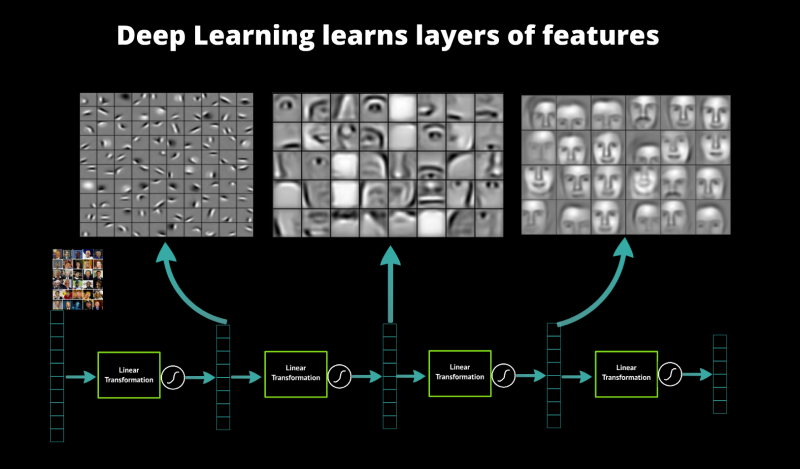
\includegraphics[width=0.85\linewidth]{lectures/01-a/dl_features.png}
% Figure from: https://www.datasciencecentral.com/profiles/blogs/a-primer-on-deep-learning
\caption{In the figure above we see how the layers closer to the input of the network are more abstract, and that those closer to the final layer are most concrete and interpretable.}
\label{fig:deep-learning-hierarchical-features}
\end{figure}

In a neural network, we feed the output of one layer onto the input of the next.
Layers are composed of linear transformations followed by non-linear activation functions.
Altogether, this system allows the network to learn the non-linear features of interest.

Hierarchical feature representations are intuitive for many domains, as our world is compositional (the whole is often a function of its parts).
For example, consider the following domains:
\begin{itemize}
    \item \textbf{Image recognition}: Pixels compose edges, which compose ``textons'' (i.e., multi-edge shapes), which compose motifs, which compose parts, which finally compose whole objects.
    Algorithms may learn to understand what an object looks like by learning a function mapping from pixels to a slightly higher level representation such as edges, then to textons, etc., until a high enough level representation is formed to represent whole objects.
    Indeed, there is evidence from neuroscience that the visual cortex represents objects in such a hierarchical manner in animals.

    \item \textbf{Language}: Language is inherently compositional as well.
    The meaning of a book is a composition of the meanings of its chapters, then paragraphs, then sentences, then phrases, then words (then even characters).
    While not all language is compositional (a ``heavy accent'' has nothing to do with weight), it often is, as language is how humans represent the world which is often compositional.

    \item \textbf{Speech}: In speech, a sample composes a band, which composes a sound, which compose phones, then phonemes, then whole words and sentences.
    The capacity for each component of this hierarchy in speech is what enables hierarchical models to represent very high-level features of sound by simply forming consecutively higher representations over what is ultimately a series of bytes.
\end{itemize}

\chapter{Hierarchical Representation}\label{chp:Hierarchical Representation}
% Authors: Hongyu (Florence) Lu, Michael Gold, Erica Dominic.
% Lecture date: 1.28.19

\section{The World as a Hierarchy}
% Authors: Hongyu (Florence) Lu, Michael Gold, Erica Dominic.
% Lecture date: 1.28.19

The world is inherently compositional and hierarchical: smaller pieces combine to form larger objects.
Humans interpret the world as a hierarchy; even the visual cortex in mammals is hierarchical in nature.

The goal of deep learning is to have a machine correctly extract hierarchical representations.
Ideally, a deep neural network should detect features at one level, then detect combinations of those features at the next level.
It is important to note that not every combination of features at one level exists in the next.

\subsection{Images}
% Authors: Hongyu (Florence) Lu, Michael Gold, Erica Dominic.
% Lecture date: 1.28.19

For example, from a patch of pixels, we want to detect edges (usually by an abrupt change in color of adjacent pixels).
From edges we can discern textons (e.g. corners, crosses).
From textons we can detect motifs, then parts of objects, and finally those parts can be pieced together to detect objects within the image.

Geometrically, if we take all $5\times5$ patches of pixels in an image, we will get a collection of $25$-dimensional vectors.
These vectors, however, would likely comprise a small (low-dimensional) part of $\mathbb{R}^{25}$.

\begin{figure}[ht]
\centering
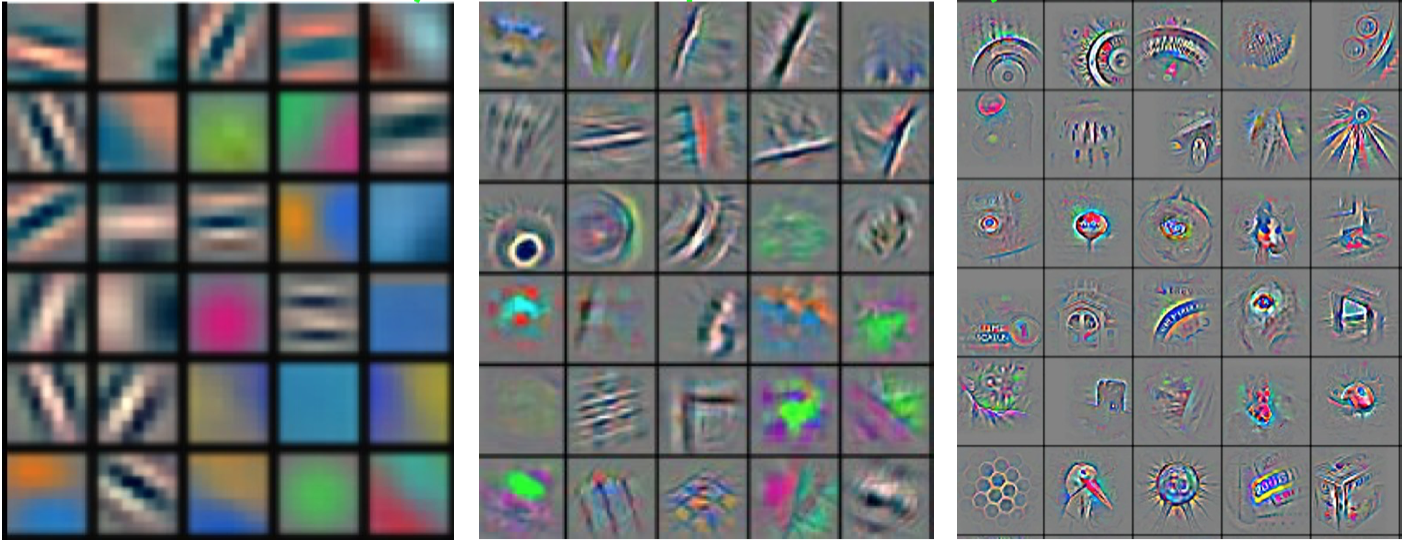
\includegraphics[width=100mm]{lectures/01-b/cnn_hierarchy.png}
\caption{Hierarchy from a convolutional neural network}
\label{fig:cnn_hierarchy}
\end{figure}

\Cref{fig:cnn_hierarchy} shows an example from a convolutional neural network.
The left pane shows detected edges, color patches, and gradients.
The middle pane has pieced those attributes together to detect textures and shapes, such as round shapes and corners.
Finally, the right pane contains discernible parts of objects.

\subsection{Text}
% Authors: Hongyu (Florence) Lu, Michael Gold, Erica Dominic.
% Lecture date: 1.28.19

The same idea can be applied to textual analysis: combinations of characters become words, combinations of words make word groups, which assemble to make clauses, which can be grouped to make sentences, and finally a collection of sentences create a story.

Again, not every combination of features at one level becomes significant in the next, e.g. not every combination of words forms a valid sentence.

\subsection{Speech}
% Authors: Hongyu (Florence) Lu, Michael Gold, Erica Dominic.
% Lecture date: 1.28.19

An audio sample is just a single number, but the frequency content of a waveform can be represented by a feature vector, and those waveforms can be pieced together to form sounds, which can then be pieced together to form syllables, etc.
Ultimately phones and phonemes are formed and pieced into words.

\chapter{Nonlinear Dimensionality Expansion}
% Authors: Hongyu (Florence) Lu, Michael Gold, Erica Dominic.
% Lecture date: 1.28.19

\section{Motivation}
% Authors: Hongyu (Florence) Lu, Michael Gold, Erica Dominic.
% Lecture date: 1.28.19

A network is ``deep'' if it has more than one stage of non-linear feature transformation. A natural question arises: why are deep networks necessary?
Theoretically, kernel machines can approximate any function with as much precision as desired.
However, that might be computationally expensive---too expensive to achieve anything in practice.

\subsection{Cover's Theorem}
% Authors: Hongyu (Florence) Lu, Michael Gold, Erica Dominic.
% Lecture date: 1.28.19

One way to rectify this problem is to bring the sample data into a higher dimension.
Thomas Cover's theorem (1965) formalized this argument.

\textbf{Cover's Theorem:} say you have a linear classifier in $N$ dimensional space with $P$ sample points, each randomly labeled with one of two class labels.
Then \cref{fig:covers_theorem} roughly illustrates the probability that these points are linearly separable.

\begin{figure}[ht]
\centering
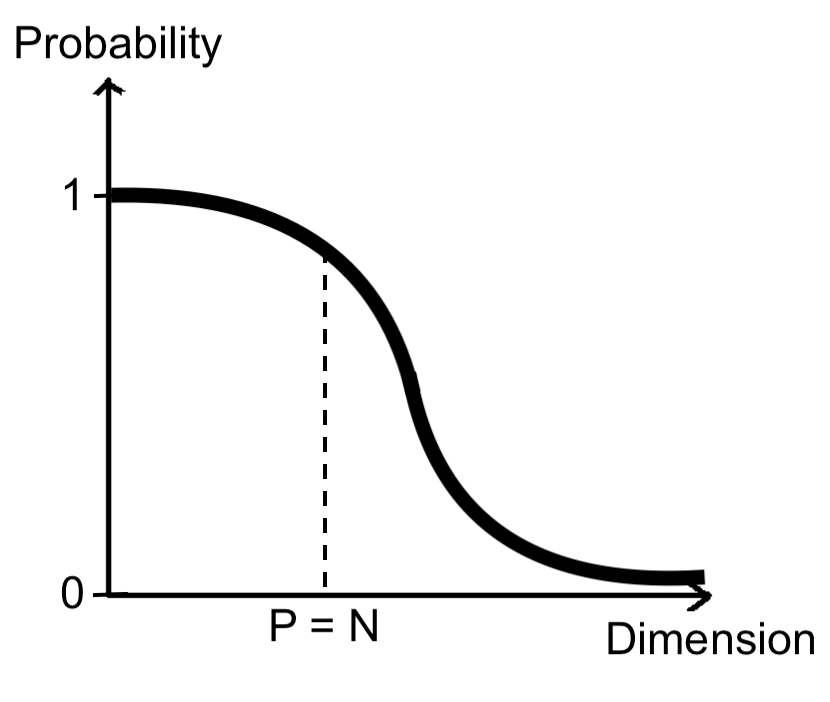
\includegraphics[width=40mm]{lectures/01-b/covers_theorem.png}
\caption{Cover's Theorem: probability of being separable vs. dimension}
\label{fig:covers_theorem}
\end{figure}

Ergo it makes sense to expand dimensionality of a representation because the data is more likely to be separable in a higher dimensional space.
One caveat: the expansion must be \emph{nonlinear}.
That brings us to deep networks, which by definition are networks with more than one nonlinear stage.

\subsection{The Manifold Hypothesis}
% Authors: Hongyu (Florence) Lu, Michael Gold, Erica Dominic.
% Lecture date: 1.28.19

Before we discuss how to expand dimensionality in a nonlinear way, we should address one concern: will working in a higher introduce an intractability problem?
The manifold hypothesis suggests that it will not pose a problem.
The manifold hypothesis postulates that natural data in high-dimensional space generally has a low-dimensional structure (see \cref{chp: manifold_hypothesis} for further discussion).
The shape of that low-dimensional space is dictated by the intrinsic factors of variation in the data, and our ideal feature extractor would extract those factors of variation.

\section{How to Expand Dimensionality Nonlinearly}\label{sec: expand_dim}
% Authors: Hongyu (Florence) Lu, Michael Gold, Erica Dominic.
% Lecture date: 1.28.19

As described in the previous section, Cover's theorem and the manifold hypothesis urge us to expand the dimension of the representation (nonlinearly) and explore it in higher dimensional space.
This is the pipeline for nonlinear dimensionality expansion:
\begin{enumerate}
    \item Linearly expand the dimension (this can be done by multiplying by matrix with more rows than columns)
    \item Apply a nonlinear transformation to each component of the vector
    \item Compress the data back into a smaller dimension (linearly or with pooling) 
\end{enumerate}

\Cref{fig:nonlinear_expansion} illustrates the process of nonlinear dimensionality expansion.
Between the first and second pane, the data is projected into higher-dimensional space linearly (observe the three-dimensional axes) and transformed nonlinearly.
Between the second and third pane, the data is brought back down to a smaller dimension (observe the two-dimensional axes) via pooling/aggregation.

\begin{figure}[ht]
\centering
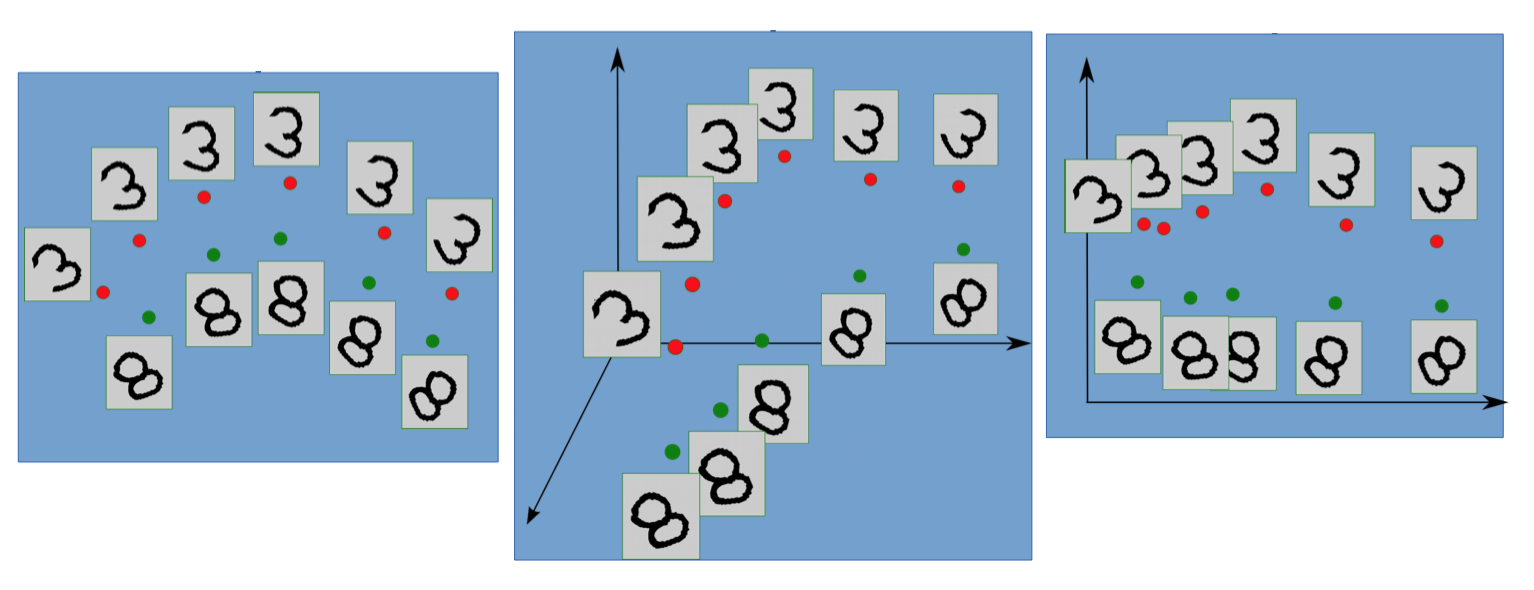
\includegraphics[width=90mm]{lectures/01-b/nonlinear_expansion.png}
\caption{Nonlinear dimensionality expansion}
\label{fig:nonlinear_expansion}
\end{figure}

\section{In the Context of the Deep Learning System Architecture}
% Authors: Hongyu (Florence) Lu, Michael Gold, Erica Dominic.
% Lecture date: 1.28.19

\Cref{sec: expand_dim} outlined the process of expanding dimensionality in a nonlinear fashion.
Here are those same steps again, this time in the context of the overall architecture for a deep learning system:
\begin{enumerate}
    \item Begin with a representation of input data
    \item Normalize the input (mean $= 0$, standard deviation $= 1$)
    \item Linearly expand the dimension (this can be done by multiplying by matrix with more rows than columns)
    \item Apply a nonlinear transformation to each component of the vector
    \item Compress the data back into a smaller dimension (linearly or with pooling) 
\end{enumerate}
This process can be repeated multiple times.

\chapter{Deep Supervised Learning: A Modular Approach}
% Authors: Hongyu (Florence) Lu, Michael Gold, Erica Dominic.
% Lecture date: 1.28.19

\section{Supervised Learning}\label{sec: supervised learning}
% Authors: Hongyu (Florence) Lu, Michael Gold, Erica Dominic.
% Lecture date: 1.28.19

\textbf{Supervised learning} is the process of improving prediction accuracy of some differentiable parameterized function (\textbf{module}) $G$ by learning from discrepancies between predicted and expected outputs.
As an illustration (see \cref{fig:supervised}), suppose we would like to train a function $G(x,w)$, where $x$ is the input variable and $w$ is a parameter called \textbf{weight}.
Say we have an input-output pair $(x,y)\in \mathbb{R}^2$.
The function $G(x,w)$ first takes the value of $x$ and predicts an output $\bar{y}$.
Then, the \textbf{cost function} $C(\bar{y},y)$ measures the distance between the predicted output $\bar{y}$ and the expected output $y$ and returns a \textbf{cost}, that is, a scalar value indicating error in prediction.
Finally, the weight $w$ will be adjusted according to the cost by using a method called \textbf{stochastic gradient descent}. 

Some examples of modules can be found in \cref{ssc:Module Classes}. 

\begin{figure}[ht]
\centering
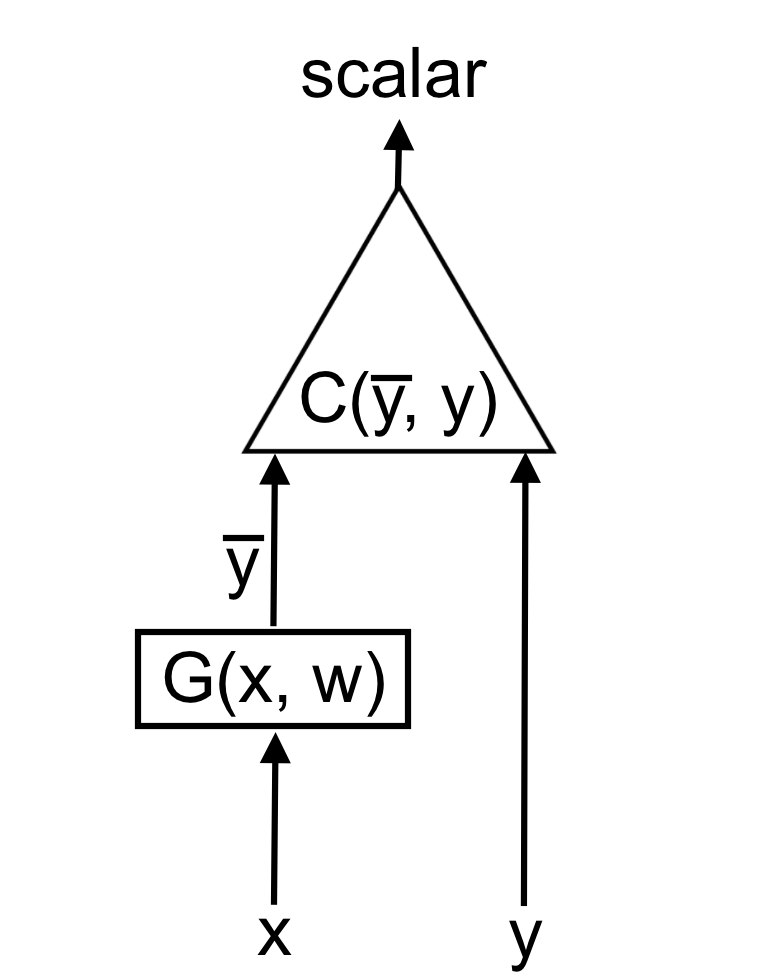
\includegraphics[width=30mm]{lectures/01-b/supervised.png}
\caption{Supervised learning}
\label{fig:supervised}
\end{figure}

\section{Stochastic Gradient Descent}\label{sec: SGD}
% Authors: Hongyu (Florence) Lu, Michael Gold, Erica Dominic.
% Lecture date: 1.28.19

Suppose we are given a training data set consisting of $P$ pairs of $N$-feature inputs and their associated outputs $(\vect{x^i}, y^i)$, where $i \in [1, P], x\in \mathbb{R}^N$, and $y\in \mathbb{R}$.
We would like to optimize the weights $\vect{w}\in \mathbb{R}^N$ of some function according to errors produced by an \textbf{objective function}:
\[
L(\vect{x^i}, y^i, \vect{w}) = C(G(\vect{x^i}, \vect{w}), y^i).
\]
Recall that \textbf{gradient descent} calculates the derivative of the cost function in attempt to find minimal cost.
If we compute the gradient for the entire training set, it may be too computationally expensive for very large training sets.
Instead, a more efficient method is adopted called \textbf{stochastic gradient descent}.
This method first evaluates the gradient randomly at the $i^\text{th}$ pair of input and output, then $\vect{w}$ is updated accordingly with a \textbf{learning rate} $\eta$:
\begin{equation}\label{eq: SGD}
\vect{w} \leftarrow \vect{w} - \eta \left[ \frac{\partial L(\vect{x^i}, y^i, \vect{w})}{\partial \vect{w}} \right]^\top.
\end{equation}
The result is a row vector consisting of $N$ partial derivatives with respect to each component of $\vect{w}$:
\[
\left[ \frac{\partial L(\vect{x^i}, y^i, \vect{w})}{\partial \vect{w}} \right]^\top = \left[ \hspace{2mm} \frac{\partial L}{\partial w_1} \hspace{2mm} \frac{\partial L}{\partial w_2} \hspace{2mm} \cdots \hspace{2mm} \right].
\]
These partial derivatives are then evaluated using a method called \textbf{backpropagation}, which will be introduced in \cref{ssc: Compute SGD using backprop}.

\section{Multi-layer Neural Network}\label{sec: Systems with Multiple Modules}
% Authors: Hongyu (Florence) Lu, Michael Gold, Erica Dominic.
% Lecture date: 1.28.19

The above supervised learning algorithm uses only one module to predict outputs $\bar{y}$.
Often, we can build a complex learning machine by assembling modules into networks.
\Cref{fig: multimodule_cascade} illustrates a simple example of a multimodule system.
This system has a \textit{cascade}, or \textit{sequential}, architecture, that is, a structure where no cycles are formed in the network and the input $X$\footnote{We simplify notations for $X$, $W$, and $Y$ in the rest of Chapter 4 since the following abstract analysis on the structure and the gradient of a multi-layer neural network applies to scalars, vectors, or matrices of the same dimension.} is passed forward in only one direction.
We can use a recurrence equation to represent a system with $n$ modules:
\[
X_i = F_i(X_{i-1}, W_i)
\]
for all $i \in [1, n]$.
Here, each module $F_i$ is an object containing trainable parameters $W_i$.
The output of the $(i-1)^\text{th}$ module $X_{i-1}$ is returned and stored internally.
It is then taken as the input for the $i^\text{th}$ module $F_i$ and so on until the signal $X_0$ reaches the last module $F_n$ and computes the predicted output $X_n$.

\begin{figure}[ht]
\centering
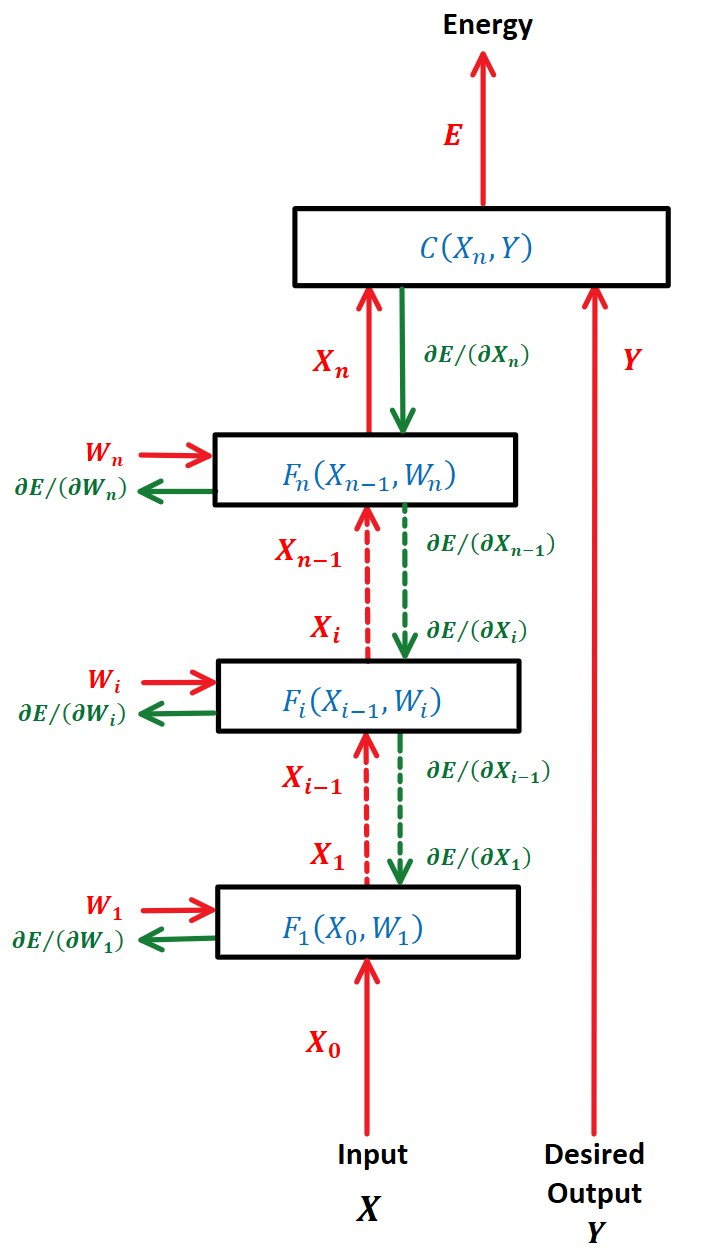
\includegraphics[width=70mm]{lectures/01-b/multimodule_cascade.jpg}
\caption{Multimodule cascade/sequential system}
\label{fig: multimodule_cascade}
\end{figure}

Similar to a single module system, the objective function $E$ is the cost function:
\[
E(Y, X_0, W) = C(X_n, Y)
\]
which measures the distance between the predicted output $X_n$ of and the desired output $Y$. 
\section{Backpropagation}\label{sec: Backpropagation}
% Authors: Hongyu (Florence) Lu, Michael Gold, Erica Dominic.
% Lecture date: 1.28.19

Recall that a learning algorithm is considered ``deep'' if it has more than one nonlinear layer.
A multimodule system with a sequential structure is often called a \textbf{multi-layer feedforward neural network}, or a \textbf{deep neural network}.
See an example of defining a two-layer neural network in PyTorch in \cref{sec: Multilayer Neural Network}.
In PyTorch, as the signal of the initial input $X_0$ propagates through a sequence of approximation functions $F_i$, PyTorch instantaneously generates another function internally, called \textbf{backpropagation}, which propagates the cascade of modules backwards in order to compute gradients discussed in \cref{sec: SGD}. 

\subsection{Compute Gradient Using Backpropagation}\label{ssc: Compute SGD using backprop}
% Authors: Hongyu (Florence) Lu, Michael Gold, Erica Dominic.
% Lecture date: 1.28.19

To compute the gradient of the objective function $E(W,Y,X)$ in an $n$-layer neural network, first consider a module $F_k$ in the network, where $k\in (0, n)$.
The forward propagation method uses the input $X_{k-1}$ produced by the $(k-1)^{\text{th}}$ module and computes a predicted output $X_k$ using the weight $W_k$, 
\[ X_k=F_k(X_{k-1},W_k). \]
Suppose we know the gradient $\frac{\partial E}{\partial X_k}$ of the cost function with respect to the output of the $k^\text{th}$ module.
That is, for each component of $X_k$, we know how much $E$ wiggles if we wiggle that component of $X_k$.
As mentioned in \cref{sec: supervised learning}, since the goal is to optimize weight $W_k$, we would like to know how much $E$ wiggles if we wiggle each component of $W_k$, namely, the gradient $\frac{\partial E}{\partial W_k}$ of the cost function with respect to the weight of the $k^\text{th}$ module.
To do so, we can simply apply \textit{chain rule} using $\frac{\partial E}{\partial X_k}$: 
\[
\frac{\partial E}{\partial W_k} = \frac{\partial E}{\partial X_k} \frac{\partial F_k(X_{k-1},W_k)}{\partial W_k}.
\]
In particular, each element $(p,q)$ of the matrix indicates how much the $p^\text{th}$ output wiggles when we wiggle the $q^\text{th}$ weight:
\[
\left[ \frac{\partial F_k(X_{k-1},W_k)}{\partial W_k} \right]_{pq} = \frac{[\partial F_k(X_{k-1},W_k)]_p}{\partial [W_k]_q}.
\]
Then, using the same method, we compute the gradient $\frac{\partial E}{\partial X_{k-1}}$ of the cost function with respect to the input of the $k^\text{th}$ module in order to pass the signal to the $(k-1)^\text{th}$ module for it to repeat the above process again.
The chain rule is applied:
\[
\frac{\partial E}{\partial X_{k-1}} = \frac{\partial E}{\partial X_k} \frac{\partial F_k(X_{k-1},W_k)}{\partial X_{k-1}}.
\]
Note that 
\[
\frac{\partial F_k(X_{k-1},W_k)}{\partial W_k}, \frac{\partial F_k(X_{k-1},W_k)}{\partial X_{k-1}}
\]
are the \textbf{Jacobian matrices} of the module $F_k$ with respect to  $W_k$ and $X_{k-1}$.

The entire process of recursively calculating gradients $\frac{\partial E}{\partial X_{i-1}}$ and $\frac{\partial E}{\partial W_i}$ starting from the $n^\text{th}$ module backwards to the first module in the network is called \textbf{backpropagation}, that is (see \cref{fig: multimodule_cascade}),

\begin{align*}
 \frac{\partial E}{\partial X_n} &= \frac{\partial C(X_n, Y)}{\partial X_n}\\
 \frac{\partial E}{\partial X_{n-1}} &=\frac{\partial E}{\partial X_n} \frac{\partial F_n(X_{n-1},W_n)}{\partial X_{n-1}} \\  
 \frac{\partial E}{\partial W_n} &=\frac{\partial E}{\partial X_n} \frac{\partial F_n(X_{n-1},W_n)}{\partial W_n} \\
 &\vdots\\ 
 \frac{\partial E}{\partial X_{i-1}} &=\frac{\partial E}{\partial X_i} \frac{\partial F_n(X_{i-1},W_i)}{\partial X_{i-1}} \\  
 \frac{\partial E}{\partial W_i} &=\frac{\partial E}{\partial X_i} \frac{\partial F_i(X_{i-1},W_i)}{\partial W_i} \\
   &\vdots\\ 
 \frac{\partial E}{\partial X_0} &=\frac{\partial E}{\partial X_1} \frac{\partial F_n(X_0,W_1)}{\partial X_0} \\  
 \frac{\partial E}{\partial W_1} &=\frac{\partial E}{\partial X_1} \frac{\partial F_1(X_0,W_1)}{\partial W_1} \\
\end{align*}

\subsection{Some Module Classes}\label{ssc:Module Classes}
% Authors: Hongyu (Florence) Lu, Michael Gold, Erica Dominic.
% Lecture date: 1.28.19

Several module classes are discussed here along with their respective gradients as they some of the most commonly used modules to build a multi-layer neural network.

\textbf{Cost module}.
A typical cost module is a squared distance function $C=\|\bar{Y}-Y\|^2$ which measures the distance between predicted and expected outputs.
It is mostly used to indicate errors in prediction.

\textbf{Linear module}.
A linear module is a function $Y=W\cdot X$ which predicts an output $Y$ by multiplying a Jacobian matrix $W$ by the input $X$.
The gradients of the cost function with respect to input and weight are 
\begin{align*}
    \frac{\partial C}{\partial X} &= W^\top \cdot \frac{\partial C}{\partial Y} \\
    \frac{\partial C}{\partial W} &= W^\top \cdot \frac{\partial C}{\partial Y} 
\end{align*}
respectively.

\textbf{ReLU module}.
A Rectifier Linear Unit(ReLU) is a pointwise nonlinearity $Y=ReLU(X)$ which takes an input $X$ and returns the identity function $Y=X$ if $X\geq0$ and $0$ if $X<0$.
The gradient is 
\[
    \frac{\partial C}{\partial X} =
    \begin{cases}
     \frac{\partial C}{\partial Y}, &\text{if } X\geq 0 \\
      0 , &\text{otherwise}
    \end{cases}
\]

\textbf{Duplicate module}.
A duplicate module $Y_1=X, Y_2=X$ makes two copies of the input $X$ and return two identical outputs $Y_1$ and $Y_2$.
The gradient with respect to the input for this module is 
\[
\frac{\partial C}{\partial X} = \frac{\partial C}{\partial Y_1} + \frac{\partial C}{\partial Y_2}
\]
since two costs are adjusted when we adjust the weight of the function.

\textbf{Add module}.
An add module $Y=X_1+X_2$ is a simple addition on two inputs $X_1$ and $X_2$.
If we adjust the weight of the function, only one cost will be adjusted.
Therefore, the gradients of the inputs are the same
\[
\frac{\partial C}{\partial X_1} = \frac{\partial C}{\partial Y} = \frac{\partial C}{\partial X_2}
\]

\textbf{Max module}.
A max module $Y = \max(X_1, X_2)$ compares inputs $X_1$ and $X_2$ and returns the larger of the two.  
The gradients with respect to $X_1$ and $X_2$ are as follows:
\[
    \frac{\partial C}{\partial X_1} =
    \begin{cases}
     \frac{\partial C}{\partial Y}, &\text{if } X_1 > X_2 \\
      0 , &\text{otherwise}
    \end{cases} \hspace{5mm},\hspace{5mm}
    \frac{\partial C}{\partial X_2} =
    \begin{cases}
     \frac{\partial C}{\partial Y}, &\text{if } X_1 < X_2 \\
      0 , &\text{otherwise}
    \end{cases}
\]

\textbf{LogSoftMax module}.
A LogSoftMax module given by
\[
Y_i=\log\left(\frac{\exp{(X_i)}}{\sum_j\exp{(X_j)}}\right) = X_i - \log\left(\sum_j\exp{(X_j)}\right)
\]
normalizes the given input $X$ to a probability distribution indicating the likelihood in $[0,1]$.
The gradient is computed as follows:
\[    
\frac{\partial C}{\partial X_i}=\frac{\partial C}{\partial Y_i} - \frac{\exp{X_i}}{\sum_j \exp{X_j}} \frac{\partial C}{\partial Y_k}
\]
Note that the gradient differs when $i=k$ and $i\neq k$.
%%%%%%%%%%%%%%%%%%%%%%%%%%%%%%%%%%%%%%%%%%
\part{Practice}\label{prt:practice}
%%%%%%%%%%%%%%%%%%%%%%%%%%%%%%%%%%%%%%%%%%
\chapter{The Manifold Hypothesis}\label{chp: manifold_hypothesis}
% Authors: Hongyu (Florence) Lu, Michael Gold, Erica Dominic.
% Lecture date: 1.28.19

\section{Facial Expressions Thought Experiment}
% Authors: Hongyu (Florence) Lu, Michael Gold, Erica Dominic.
% Lecture date: 1.28.19

Say we have infinitely many pictures of a person making all possible facial expressions.
Each image is $2000 \times 1000$ pixels and has $3$ color channels, so each image is $6,000,000$-dimensional vector.

The set of all images is a small subset of $6,000,000$-dimensional space.
What does that subset look like?
What is the dimensions of the surface?
On a patch of that surface, how many dimensions can you move and still stay on that surface?

That surface is a manifold (roughly speaking, a continuous surface).
Moreover, it is limited by the number of degrees of freedom in the human face, which is bounded above by the number of muscle groups a person can control in his face.
Ergo that subset of $\mathbb{R}^{6000000}$ is relatively low-dimensional.

This thought experiment illustrates the manifold hypothesis, which postulates that natural data in high dimensional space generally has a low dimensional structure.
\chapter{Tensor Transformations}
% Authors: Dustin Godevais , Reuben Juster, Yi Li,. 2/5/18.

The following sections summarize and visualize how you can transform data represented in matrix form. 
Input data can be defined as a matrix with the $i^{th}$ row corresponding to the $i^{th}$ data point and each additional columns representing a new dimension of the data.
$\matr{X}$ in the below examples is an input matrix with 1000 data points and two dimensions whose values are standard normally distributed. 
In the following figures, data points are colored according to their original $x_{N,1}$  dimension violet to yellow for negative to positive values.

\[
\matr{X} =
\begin{bmatrix}
    x_{1,1} & x_{1,2} \\
    x_{2,1} & x_{2,2} \\
    x_{3,1} & x_{3,2} \\
    \vdots & \vdots  \\
    x_{1000,1} & x_{1000,2}
\end{bmatrix}
\]

\begin{figure}[H]
\begin{center}
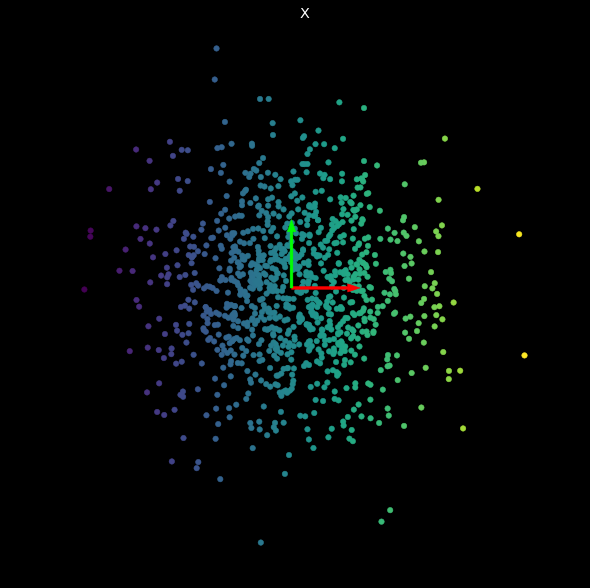
\includegraphics[width=200pt]{labs/01/images/standardnormal.png}
\end{center} 
\caption{Original $\matr{X}$ Visualized}
% \label{fig:mon}
\end{figure}

\section{Linear Transformations}
% Authors: Dustin Godevais , Reuben Juster, Yi Li,. 2/5/18.
There are several linear transformation that can be executed on $\matr{X}$ including:

\begin{itemize}
% \tightlist
\item
Rotation (\(\matr{U}\))

\item
Scaling \((s_1, s_2)\)

\item
Reflection (\(\matr{V}\))
\item
Shearing
\item
Translation
\end{itemize}

The product of the first three form weights as shown below.

\[
\matr{W} = \matr{U}
\begin{bmatrix}
    s_1 & 0 \\
    0 & s_2 
\end{bmatrix}
\matr{V}^\top
\]


\subsection{Rotation}
During rotation, each point is rotated about the origin by the indicated angle. 
The below equation populates $\matr{U}$ based on rotating points by \(\theta\) counter-clockwise.

\[
\matr{U} = 
\begin{bmatrix}
    \cos(\theta) & \sin(\theta)\\
    \sin(\theta) & -\cos(\theta)
\end{bmatrix}
\]

Keeping scaling and reflection constant, the below figure shows a set up points with different  \(\theta\)s .

\begin{figure}[H]
\begin{center}
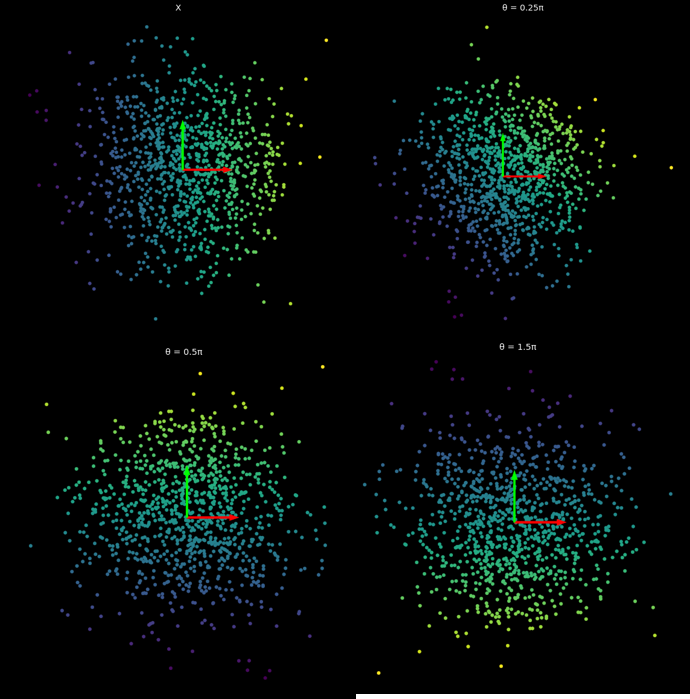
\includegraphics[width=300pt]{labs/01/images/Rotation.png}
\end{center} 
\caption{Rotation Visualized}
% \label{fig:mon}
\end{figure}
% \FloatBarrier


\subsection{Scaling}
Scaling the points expands or contracts the points about the origin. 
This controlled separately for each dimension by \(s_1\) and \(s_2\) .

\begin{figure}[H]
\begin{center}
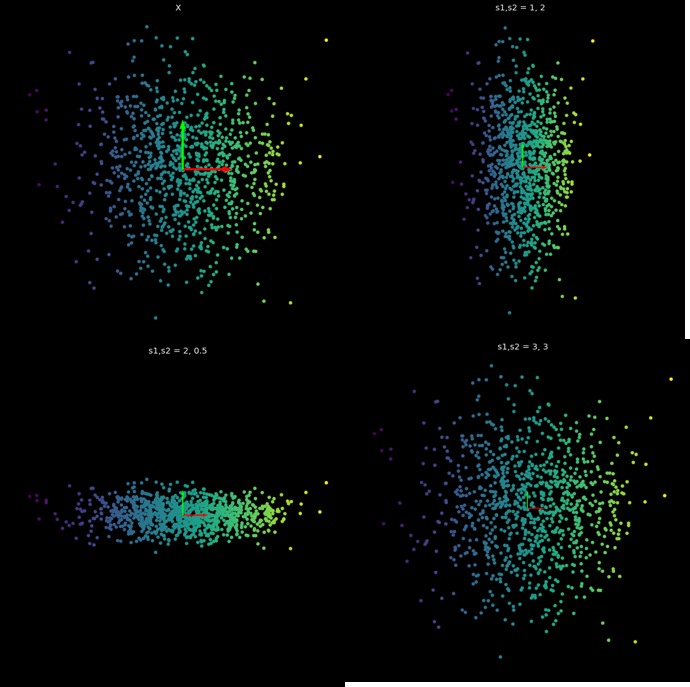
\includegraphics[width=300pt]{labs/01/images/Scaling.png}
\caption{Scaling Visualized}
% \label{fig:mon}
\end{center} 
\end{figure}
% \FloatBarrier


\subsection{Reflection}
Reflecting points projects them on the other side of a defined line that crosses the origin. 
The line that goes from the original point to the projected point is perpendicular to the defined line, and the intersection to the defined line is the midpoint.


\begin{figure}[H]
\begin{center}

\includegraphics[width=200pt]{labs/01/images/reflection_example.png}
\end{center} 
\caption{Reflection Defined}
% \label{fig:mon}
\end{figure}
% \FloatBarrier


\(\matr{V}\) can be defined by

\[
\matr{V} = 
\begin{bmatrix}
    \cos(2\theta) & \sin(2\theta)\\
    \sin(2\theta) & -\cos(2\theta)
\end{bmatrix}
\]

Where the defined line is \(x_2 = \tan(\theta) x_1 \)

\begin{figure}[H]
\begin{center}
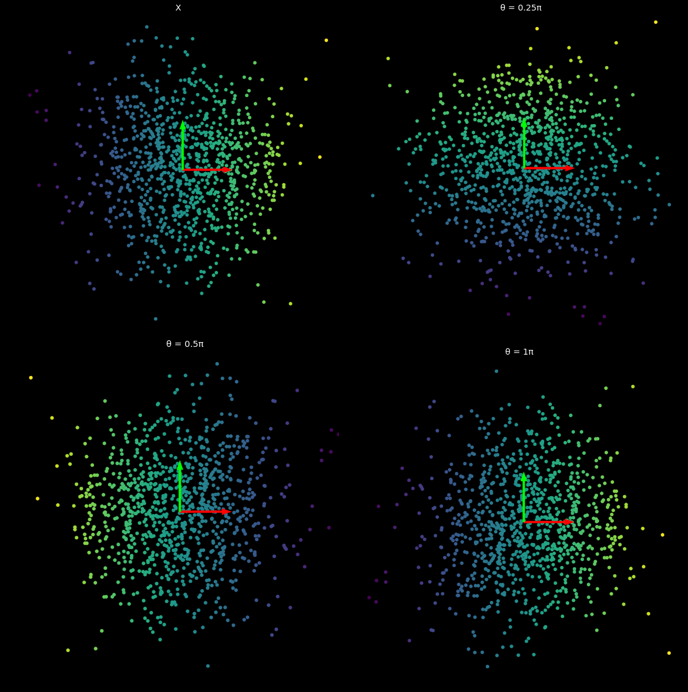
\includegraphics[width=400pt]{labs/01/images/Reflection.png}
\end{center} 
\caption{Reflection Visualized}
% \label{fig:mon}
\end{figure}
% \FloatBarrier

\subsection{Shearing}
Shearing points, which is separate from the weight calculation, shifting points in one dimension proportional to their value in the other dimension.

\(\matr{Y} = \matr{X}  \begin{bmatrix}
    1 & k\\
    0 & 1
\end{bmatrix} \) 
Shift points on the \(x_1\) dimension proportional to the \(x_2\) dimension

\(\matr{Y} = \matr{X}  \begin{bmatrix}
    1 & 0\\
    k & 1
\end{bmatrix} \)
Shift points on the \(x_2\) dimension proportional to the \(x_1\) dimension

\begin{figure}[H]
\begin{center}
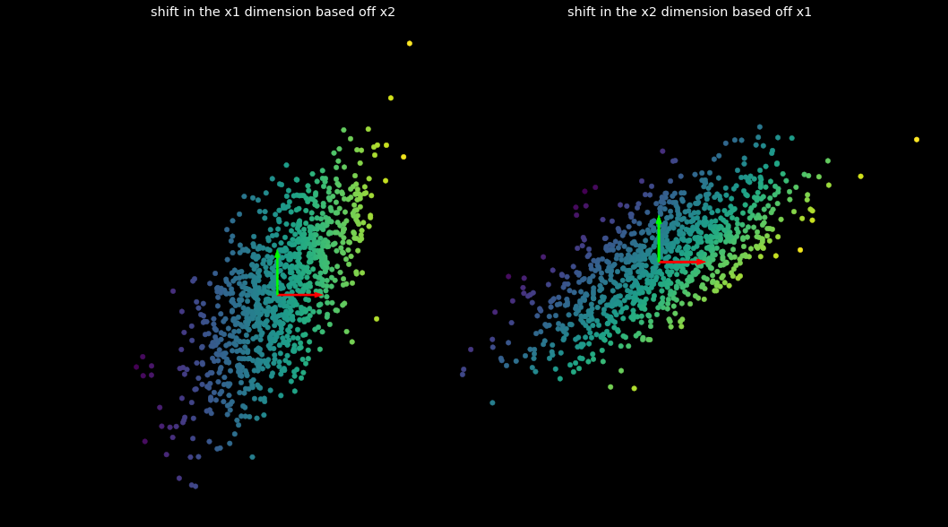
\includegraphics[width=400pt]{labs/01/images/shear.png}
\end{center} 
\caption{Shear Visualized}
% \label{fig:mon}
\end{figure}
% \FloatBarrier

\subsection{Translation}
The translation of points, which is separate from the weight calculations moves them uniforming in the direction indicated.

\[ \matr{Y} = \matr{X} 
+ \begin{bmatrix}
    1 & 1 \\
    1 & 1 \\
    1 & 1 \\
    \vdots & \vdots  \\
    1 & 1
\end{bmatrix}
\begin{bmatrix}
    t_1 & 0\\
    0 & t_2
\end{bmatrix} \] 
(Shift points left or right by \(t_1\) and up or down by  \(t_2\) dimension)

\begin{figure}[H]
\begin{center}
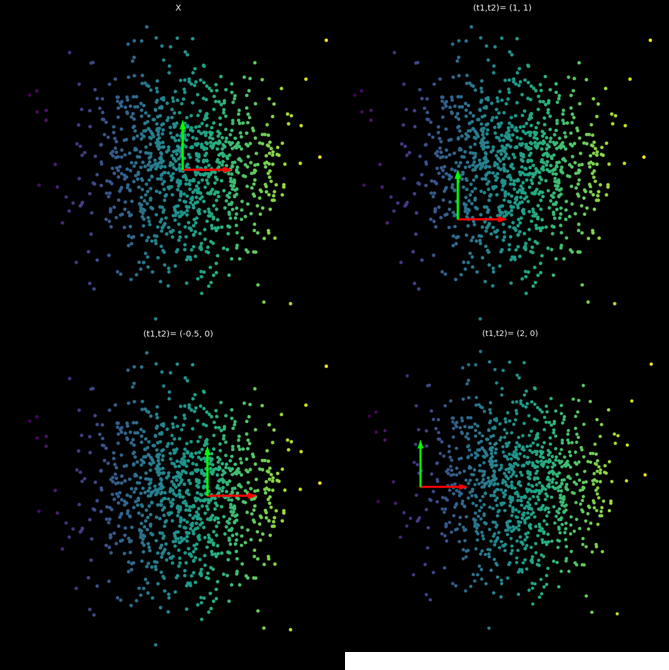
\includegraphics[width=400pt]{labs/01/images/translation.png}
\end{center} 
\caption{Translation Visualized}
% \label{fig:mon}
\end{figure}
% \FloatBarrier

\section{Non-Linear Transformations}
% Authors: Dustin Godevais , Reuben Juste, Yi Li,. 2/5/18.
Linear transformations are capable of altering data in many different ways, but linear transformations cannot curve data. 
That is where non-linear transformations come in. There are several types of non-linear transformations such as:

\begin{itemize}
% \tightlist
\item
Rectified linear unit (ReLU) - \(y = x_1\) if \(x_1 > 0\) else $0$ 
\item
Polynomial- \(y = x_1^2\) or \(y = x_1 x_2\)
\item
Step - \(y = 1\) if \(x > 0 \) else $0$ 

\end{itemize}

One of the most common non-linear transformations is the hyperbolic tangent, which in the context of 2D Tensors can be applied as below:
\[f(x) = \tanh(
\begin{bmatrix}
s & 0\\
0 & s
\end{bmatrix}
x)\]

This function first stretches out the points using scalar $s$ via scaling, then the hyperbolic tanget squashes the points into a square.
The larger $s$ is, the more points end up in the square.

\begin{figure}[H]
\begin{center}
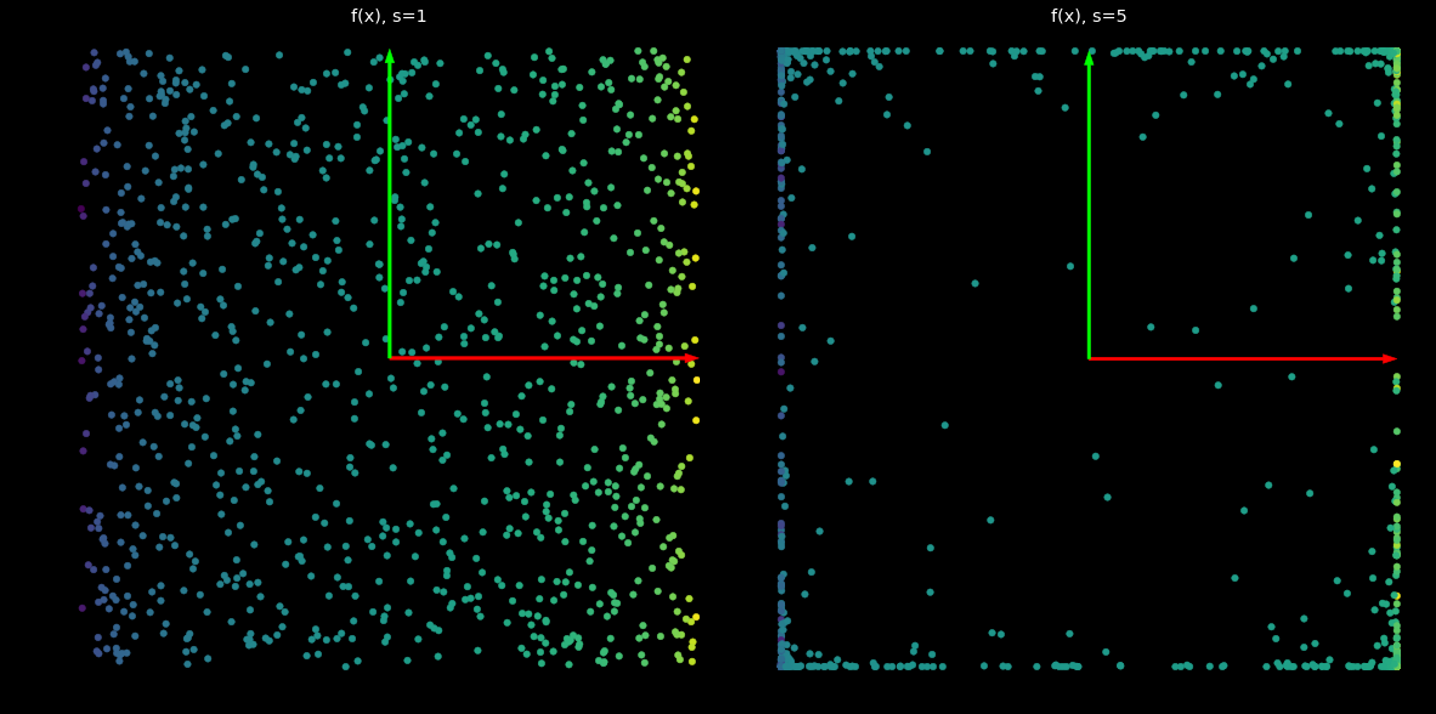
\includegraphics[width=400pt]{labs/01/images/tanh.png}
\end{center} 
\caption{Tanh in Isolation}
% \label{fig:mon}
\end{figure}
% \FloatBarrier

Tanh can create curved surfaces when it is sandwiched in-between two linear transformations in a three layer neural network.

\begin{figure}[H]
\begin{center}
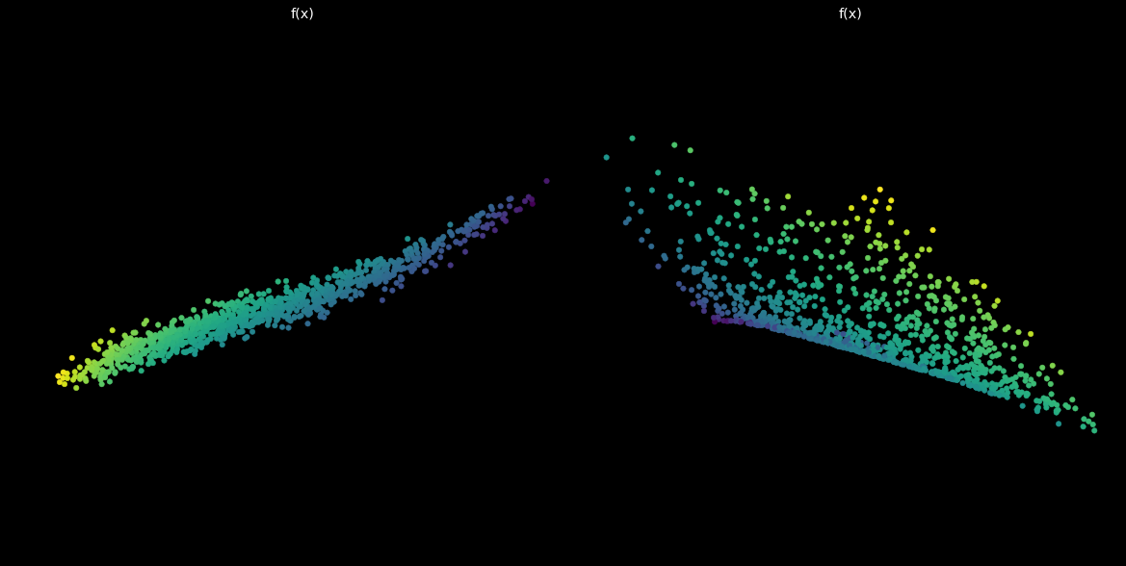
\includegraphics[width=400pt]{labs/01/images/tanh_sandwich.png}
\end{center} 
\caption{Tanh In-Between Two Linear Layers}
% \label{fig:mon}
\end{figure}
% \FloatBarrier


\chapter{Convolutional Nets}
% Authors: Fekade Brook, Nicholas Greenquist, Aaron Wong
% Lecture date: 2/11/2019

\section{Parameter Space Transform}
% Authors: Fekade Brook, Nicholas Greenquist, Aaron Wong
% Lecture date: 2/11/2019

Weights of a neural net do not necessarily have to be parameters. 
They can be outputs of other functions.

\begin{figure}
    \centering
    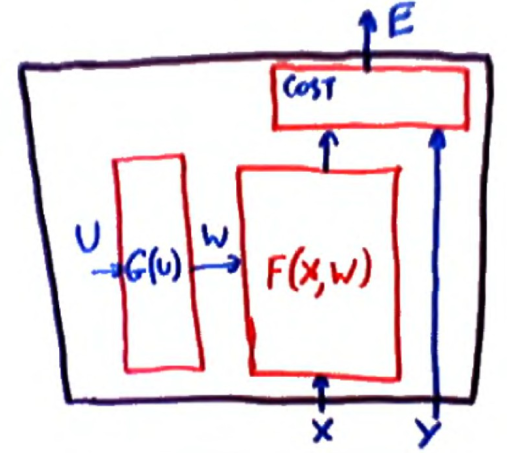
\includegraphics[width=150pt]{lectures/03-a/images/parameterize.png}
    \caption{Re-parameterization of weight parameters U}
    \label{fig:param}
\end{figure}

For example, in \cref{fig:param} the parameters of $F$ are $W$ but $W$ are not the parameters that you learn. 
The parameters that you learn are the $U$ but these are re-parameterized by a function $G:U\rightarrow W$ before being sent to $F$. 
This is only simple example of re-parameterizing. 
We could also have a function that re-paramterizes the inputs $X$.

If you use the functional form of PyTorch this is very easy to do. 
Everything works when you backpropagate. 
To use the above figure as an example again, when you back propagate you get the gradient of the cost with respect to the $F$ module. 
Backpropagating even further gives you the Jacobian of $F$ module times the Jacobian of the $G$ module. 
The nice thing is that if you use PyTorch, all of the gradients and backpropagation is handled for you and you do not need to think about it. 

\section{Weight Sharing}
% Authors: Fekade Brook, Nicholas Greenquist, Aaron Wong
% Lecture date: 2/11/2019

\Cref{fig:sharing} is an example of a function $G$ that can be used to re-parameterize the weight parameters.

\begin{figure}
    \centering
    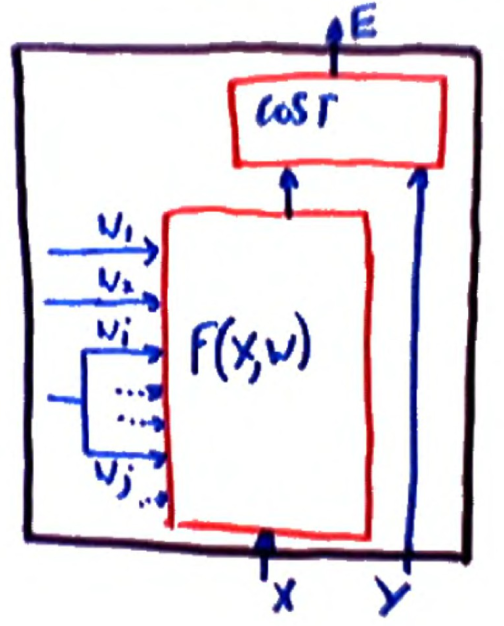
\includegraphics[width=150pt]{lectures/03-a/images/weight_sharing.png}
    \caption{Weight sharing of weights $w_{i}$}
    \label{fig:sharing}
\end{figure}

In this example, $G$ replicates a single parameter multiple times and passes the new parameters to $F$. 
When we backpropagate, the gradient with respect to that shared parameter is equal to the sum of the gradients with respect to each of the replicated parameters.

\section{Mixture of Experts}
% Authors: Fekade Brook, Nicholas Greenquist, Aaron Wong
% Lecture date: 2/11/2019

If we have a function that works well in restricted domains of the input space but does not work globally, we want to create something that is called a Mixture of Experts. 
This idea of combining multiple, local optimal functions allows for very interesting architectures. 
This idea is actually the inspiration behind attention mechanisms that we will see later. 

Imagine you have a problem with 3 distinct types of inputs. 
An example is recognizing faces. 
You might need a different model for children, male adults, and female adults. 
You would want 3 expert models for each of those types.

Visually, we can see that this input would benefit from 3 separate classifiers that we can combine in \cref{fig:mixture}

\begin{figure}
    \centering
    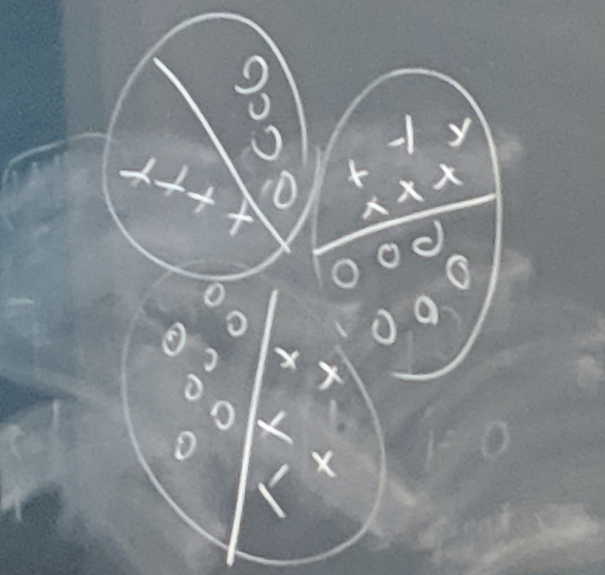
\includegraphics[width=200pt]{lectures/03-a/images/mixture.png}
    \caption{Mixture of 3 separate classifiers}
    \label{fig:mixture}
\end{figure}

The goal is to turn non-linear problems into a mixture of multiple linear classifiers. 
The mixture's sole job is to now decide where the regions are. 
Often times each of the expert systems is a neural net itself and is combined using a neural net to decide optimal region splitting. 
Softmax is often used as the final layer of a neural network for classification. 
These models can be trained with backpropagation just like what we have seen so far. 

A good example of this is speech recognition. 
Imagine I want a model to work on German, French, and English. 
I don't want to create 3 different models. 
Instead I can let the model decide which language it is dealing with and then pass the sequence into different expert systems. 
However, in reality, the input does in fact go through all of the systems, and so we use a ``Gater'' module to decide which expert to believe. 
This is all done by how our weights are tuned and how they behave with certain types of inputs. 
As usual, the modules are trained using backpropagation. 
This includes the Gater module.

\section{Time Delayed Inputs}
% Authors: Fekade Brook, Nicholas Greenquist, Aaron Wong
% Lecture date: 2/11/2019

Let's say we want to apply a neural network to a sequence of vectors. 
We want to use an input that is a "time window''. 
That is, we want to do time series predictions.

For example, you are a power company and you want to predict what the power consumption is going to be for different areas. 
The input is obviously historical power consumption and weather but you might also have time of day. 
Time-Delayed inputs are also heavily used in the financial markets. 

\begin{figure}
    \centering
    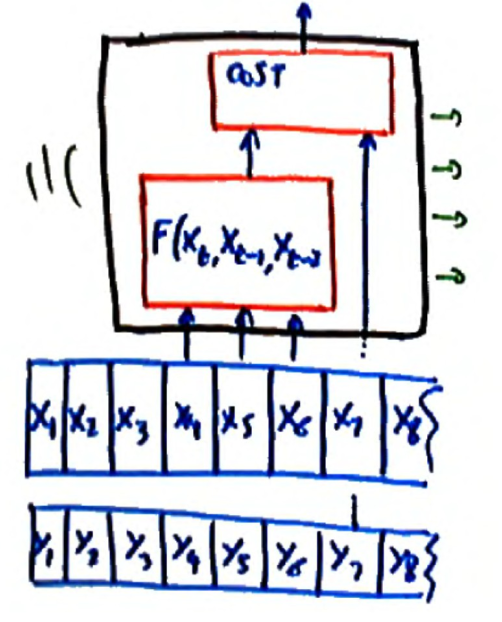
\includegraphics[width=150pt]{lectures/03-a/images/td_inputs.png}
    \caption{Neural network for time-delayed inputs}
    \label{fig:td_inputs}
\end{figure}

To do this, we feed the neural network a recent window of observed values and ask it to predict the next value. 
During training, the output at time step $t$ is usually the input at time step $t+1$ as in \cref{fig:td_inputs}. 
The motivation for this is that like in financial markets, the thing that you want to predict has already been observed. 
You just want to predict when it will happen in the future. 
The basic technique is to take our network and ``slide'' it across the inputs. 
The same weights end up getting applied to multiple inputs in the input sequence. 

An example of using time-delayed inputs is using a neural network for sound recognition on speech. 
Suppose you have a speech signal and you want to train a neural network to figure out what sound is being pronounced at the moment. 
After some pre-processing of the sound, the neural network looks at a small window of the signal. 
The network gives you a score for every possible sound that can exist. 
Slide the network over the input sequence by 10 milliseconds or so and repeat. 
Now for every 10 millisecond, you have a vector of scores for what sound is being pronounced.

\section{1D Temporal Convolutional Net}
% Authors: Fekade Brook, Nicholas Greenquist, Aaron Wong
% Lecture date: 2/11/2019

The idea we saw before of sliding the same network across different areas of the input leads to the idea of convolutions. 

Image we have the 2-layer network as shown in \cref{fig:2layer}. 
It is trying to recognize, classify or predict something from $x_{1,t}, x_{2,t}$ input sequences. 
The first layer is a single linear layer. 
Each of $C_{1}, C_{2}, C_{3}, C_{4}$ are shifted versions of the linear layer looking at different time steps of the inputs $x_{1,t}, x_{2,t}$. 
Take for instance $C_{1}$.
$C_{1}$ consists of a bunch of units each looking at a $2\times 3$ grid of the input.
After the first iteration, take those same units and shift them by one time step so that the units are now looking at a $2\times 3$ grid shifted to the right by 1.
$C_{2}$ represents this newly shifted set of units.
This is done until all the inputs are looked at.
The second layer then does something similar.
For example, in \cref{fig:2layer}, $L2$ takes three different time steps of the outputs of the units in $C_{1}, C_{2}, C_{3}, C_{4}$ and produces an output.
The important part to note here is that $C_{1}, C_{2}, C_{3}, C_{4}$ all contain the same units.
They are just the units at different time steps.

\begin{figure}
    \centering
    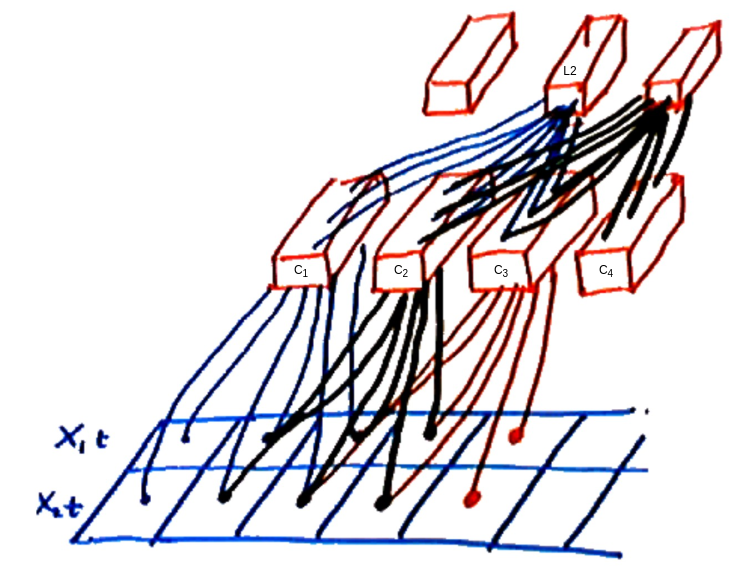
\includegraphics[width=200pt]{lectures/03-a/images/conv_net.png}
    \caption{1D (temporal) ConvNet}
    \label{fig:2layer}
\end{figure}

The idea of shared weights is that many of the weights in each layer are exactly the same but used in different time steps. 
As you train a network like this many of the parameters are used to compute values across different time steps so when you backpropagate, you need to compute the gradient of the same weight at each time step, add them up and then update that common weight with that gradient.

\subsection{2D Temporal Convolutional Net}
% Authors: Fekade Brook, Nicholas Greenquist, Aaron Wong
% Lecture date: 2/11/2019

\begin{center}
    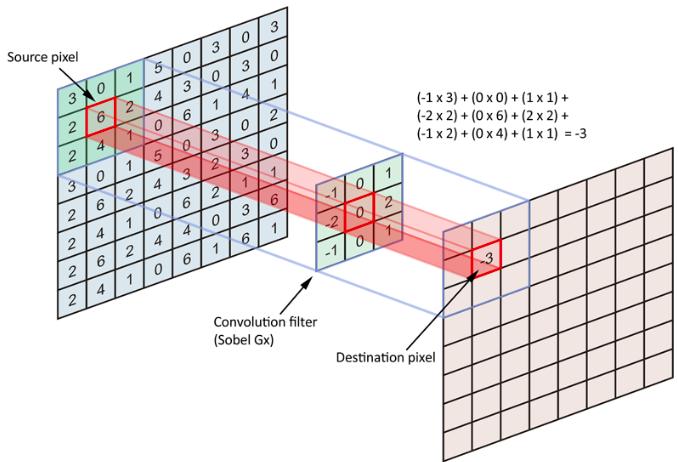
\includegraphics[width=200pt]{lectures/03-a/images/conv.png}
\end{center}

As you can see from the image above, that single filter has 9 weights. However, we slide that filter across the entire input grid. So, those 9 weights are shared to compute many different output values destination grid. When training a network with convolution like this, we need to keep track that each weight is being used multiple times and combine the gradients correctly. 

%%%%%%%%%%%%%%%%%%%%%%%%%%%%%%%%%%%%%%%%%%
\part{Coding}\label{prt:coding}
%%%%%%%%%%%%%%%%%%%%%%%%%%%%%%%%%%%%%%%%%%
\chapter{Multimodule Systems}
% Authors: Hongyu (Florence) Lu, Michael Gold, Erica Dominic.
% Lecture date: 1.28.19

\section{Multilayer Neural Network}\label{sec: Multilayer Neural Network}
% Authors: Hongyu (Florence) Lu, Michael Gold, Erica Dominic.
% Lecture date: 1.28.19

In \cref{sec: Systems with Multiple Modules}, we discussed a forward multimodule system.
The following code includes three different ways of building a two-layer neural network.

\begin{minted}{python}
    import torch 
    from torch import nn
    
    image = torch.randn(3, 10, 20)
    in_size = image.nelement()
    h_size = 60
    out_size = 6
    
    #### Functional paradigm 
    m1 = nn.Linear(in_size, h_size)
    m2 = nn.Linear(h_size, out_size)
    # forward prop
    hid = torch.relu(m1(image.view(-1)))
    out = m2(hid)
    
    #### Using containers
    model = nn.Sequential(m1, nn.relu(), m2)
    # forward prop
    out = model(image.view(-1))
    
    #### Using object oriented programming 
    class Net(nn.Module):
        def __init__(self, in_s, h_s, out_s):
            super().__init__()
            self.m1 = nn.Linear(in_s, h_s)
            self.m2 = nn.Linear(h_s, out_s)
            
        def forward(self, x):
            x = torch.relu(self.m1(x.view(-1)))
            x = self.m2(x)
            return x
            
    model = Net(in_size, h_size, out_size)
    out = model(image)
\end{minted}

First, we import torch and the \texttt{nn} module from torch in Python.
The \texttt{nn} module has several predefined modules.
The input is a random matrix of size $3 \times 10 \times 20$.
We can think of this matrix as an image with $3$ RGB components and is $10$ rows by $20$ columns.
The total size is obtained by \texttt{image.nelement()}.
Next, we build a neural network with two linear layers, which are multiplications by matrix.

Using functional paradigm, we create the first module \texttt{m1} using \texttt{nn.Linear()} and give the sizes of the input \texttt{in\_size} and output \texttt{h\_size}.
Similarly, the second module \texttt{m2}, which is also a linear module, is created with \texttt{nn.Linear()}.
It takes the vector of the same size \texttt{h\_size} and produces the vector of the output size \texttt{out\_size}, which is $6$ (a $6$-way classification).
Then, the forward propagation calls functions \texttt{m1} and \texttt{m2}.
The variable \texttt{hid} first applies the module \texttt{m1} to \texttt{image.view($-1$)}, that is, it takes the \texttt{image} and uses \texttt{view.($-1$)} to turn a $3$-dimensional tensor into a single vector.
Then, \texttt{hid} applies \texttt{ReLU} (Rectifier Linear Unit) to the single vector.
Each component of the vector is passed through a halfway rectifier.
Recall that the output of the \texttt{ReLU} function is the identity function if the argument is positive and $0$ if the argument is negative.
Lastly, we obtain the result \texttt{out} by taking the result \texttt{hid} and applying the second module \texttt{m2} to it.

Another way of building a neural network is to use containers that define certain predefined structures.
Instead of writing functions individually for each module, variable \texttt{model} uses a container, \texttt{nn.Sequential()}, to build a graph and pass the signal in the order of the input modules \texttt{m1}, \texttt{nn.ReLU()}, and \texttt{m2}.
Note that the list of modules is called a sequence.
Then, the forward propagation obtains the result \texttt{out} by taking \texttt{model} and applying \texttt{image.view($-1$)} to it.

Lastly, we can define a class using object oriented programming for this particular two-layer neural network.
First, we initiate parameters \texttt{in\_s}, \texttt{h\_s}, and \texttt{out\_s} for input and output sizes.
Then, we create two linear module \texttt{m1} and \texttt{m2} using \texttt{nn.Linear()}.
Next, the forward function first takes the input \texttt{x} and turns it into a single vector.
Then, the function applies \texttt{m1} module to the vector and applies \texttt{ReLU} to the result.
The module \texttt{m2} is then applied to the result \texttt{x}.
The variable \texttt{model} then calls the class \texttt{Net} and the variable \texttt{out} applies the \texttt{image} to the class to obtain the final result.
Note that this method is already being implemented by PyTorch.

When we run a feedforward neural network, PyTorch automatically calculates the gradient of the weight using backpropagation.
\chapter{Introduction to \emph{PyTorch} and \texttt{Tensor}s}
% Authors: Dustin Godevais , Reuben Juste, Yi Li,. 2/5/18.
    \section{What is \emph{PyTorch}?}\label{what-is-pytorch}
    % Authors: Dustin Godevais , Reuben Juste, Yi Li,. 2/5/18.
    \emph{PyTorch} is a Python based scientific computing package targeting on two sets of audiences:

   
\begin{itemize}
% \tightlist
\item
  Tensorial library that uses the power of GPUs
\item
  A deep learning research platform that provides maximum flexibility
  and speed
\end{itemize}

    
     \begin{Verbatim}[commandchars=\\\{\}]
{\color{incolor}In [{\color{incolor}1}]:} \PY{k+kn}{import} \PY{n+nn}{torch}
\end{Verbatim}

    \section{Getting help in Jupyter}\label{getting-help-in-jupyter}
    % Authors: Dustin Godevais , Reuben Juste, Yi Li,. 2/5/18.

    
%\subsection*{Jupyter Tips}
    \href{https://jupyter.org/}{Jupyter Notebook} is a common Integrated Development Environment (IDE) for deep learning. There are a few commands specific to Jupyter Notebook that are helpful for coding.   
        \subsection{Using tab}
        Tab will list all available functions, while shift + tab will open the documentation.

        \subsection{Using ?}
        \begin{Verbatim}[commandchars=\\\{\}]
{\color{incolor}In [{\color{incolor}2}]:} \PY{c+c1}{\PYZsh{} Open the documentation, same as \PYZlt{}shift\PYZgt{} + \PYZlt{}tab\PYZgt{} on \PYZsq{}torch.nn.Module()\PYZsq{}}
         torch.nn.Module\PY{o}{?}
\end{Verbatim}


    \begin{Verbatim}[commandchars=\\\{\}]
{\color{incolor}In [{\color{incolor}3}]:} \PY{c+c1}{\PYZsh{} See the source code of all functions being executed in the Module}
         torch.nn.Module\PY{o}{??}
\end{Verbatim}
        
\subsection{Dropping to Bash}
\begin{Verbatim}[commandchars=\\\{\}]
{\color{incolor}In [{\color{incolor}4}]:} \PY{c+c1}{\PYZsh{} List all the files in the current directory}
         \PY{o}{!}ls \PYZhy{}lh 
\end{Verbatim}

\begin{Verbatim}[commandchars=\\\{\}]
{\color{incolor}In [{\color{incolor}5}]:} \PY{c+c1}{\PYZsh{} Getting some general help}
         \PY{o}{\PYZpc{}}\PY{k}{magic} 
\end{Verbatim}

\section{Tensors}\label{tensors}   
% Authors: Dustin Godevais , Reuben Juste, Yi Li,. 2/5/18.
A tensor is a n-dimensional array, \emph{PyTorch} provides functions for operating on Tensors like numpy does for arrays.
\begin{Verbatim}[commandchars=\\\{\}]
{\color{incolor}In [{\color{incolor}6}]:} \PY{c+c1}{\PYZsh{} Generate a tensor of size 2x3x4}
         \PY{n}{t} \PY{o}{=} \PY{n}{torch}\PY{o}{.}\PY{n}{Tensor}\PY{p}{(}\PY{l+m+mi}{2}\PY{p}{,} \PY{l+m+mi}{3}\PY{p}{,} \PY{l+m+mi}{4}\PY{p}{)}
         \PY{n+nb}{type}\PY{p}{(}\PY{n}{t}\PY{p}{)} 
\end{Verbatim}


\begin{Verbatim}[commandchars=\\\{\}]
{\color{outcolor}Out[{\color{outcolor}6}]:} torch.Tensor
\end{Verbatim}
            
\begin{Verbatim}[commandchars=\\\{\}]
{\color{incolor}In [{\color{incolor}7}]:} \PY{c+c1}{\PYZsh{} Get the size of the tensor}
         \PY{n}{t}\PY{o}{.}\PY{n}{size}\PY{p}{(}\PY{p}{)} 
\end{Verbatim}


\begin{Verbatim}[commandchars=\\\{\}]
{\color{outcolor}Out[{\color{outcolor}7}]:} torch.Size([2, 3, 4])
\end{Verbatim}
            
\begin{Verbatim}[commandchars=\\\{\}]
{\color{incolor}In [{\color{incolor}8}]:} \PY{c+c1}{\PYZsh{} Get the dimension of the tensor, for example, 1 for vectors, 2 for matrices}
         \PY{n}{t}\PY{o}{.}\PY{n}{dim}\PY{p}{(}\PY{p}{)} 
\end{Verbatim}


\begin{Verbatim}[commandchars=\\\{\}]
{\color{outcolor}Out[{\color{outcolor}8}]:} 3
\end{Verbatim}
            
\begin{Verbatim}[commandchars=\\\{\}]
{\color{incolor}In [{\color{incolor}9}]:} \PY{c+c1}{\PYZsh{} Total number of elements in the tensor}
         \PY{n}{t}\PY{o}{.}\PY{n}{numel}\PY{p}{(}\PY{p}{)} 
\end{Verbatim}


\begin{Verbatim}[commandchars=\\\{\}]
{\color{outcolor}Out[{\color{outcolor}9}]:} 24
\end{Verbatim}
 
Note: Mind the underscore! 
Any operation that mutates a tensor in-place is post-fixed with an underscore. 
The in-place replacement will change the object. It is encouraged to perform operations in-place to optimize usage of memory.
            
\begin{Verbatim}[commandchars=\\\{\}]
{\color{incolor}In [{\color{incolor}10}]:} 
         \PY{n}{t}\PY{o}{.}\PY{n}{random\PYZus{}}\PY{p}{(}\PY{l+m+mi}{10}\PY{p}{)} 
\end{Verbatim}


\begin{Verbatim}[commandchars=\\\{\}]
{\color{outcolor}Out[{\color{outcolor}10}]:} tensor([[[4., 6., 2., 4.],
                  [8., 2., 6., 9.],
                  [1., 4., 9., 9.]],
         
                 [[8., 5., 5., 5.],
                  [4., 1., 1., 7.],
                  [4., 4., 6., 9.]]])
\end{Verbatim}
            
\begin{Verbatim}[commandchars=\\\{\}]
{\color{incolor}In [{\color{incolor}11}]:} \PY{n}{r} \PY{o}{=} \PY{n}{torch}\PY{o}{.}\PY{n}{Tensor}\PY{p}{(}\PY{n}{t}\PY{p}{)}
         \PY{c+c1}{\PYZsh{} This resizes the tensor permanently}
         \PY{n}{r}\PY{o}{.}\PY{n}{resize\PYZus{}}\PY{p}{(}\PY{l+m+mi}{3}\PY{p}{,} \PY{l+m+mi}{8}\PY{p}{)}  
         \PY{n}{r}
\end{Verbatim}


\begin{Verbatim}[commandchars=\\\{\}]
{\color{outcolor}Out[{\color{outcolor}11}]:} tensor([[4., 6., 2., 4., 8., 2., 6., 9.],
                 [1., 4., 9., 9., 8., 5., 5., 5.],
                 [4., 1., 1., 7., 4., 4., 6., 9.]])
\end{Verbatim}
            
\begin{Verbatim}[commandchars=\\\{\}]
{\color{incolor}In [{\color{incolor}12}]:} \PY{c+c1}{\PYZsh{} Replace all element in r with 0\PYZsq{}s}
         \PY{n}{r}\PY{o}{.}\PY{n}{zero\PYZus{}}\PY{p}{(}\PY{p}{)} 
\end{Verbatim}


\begin{Verbatim}[commandchars=\\\{\}]
{\color{outcolor}Out[{\color{outcolor}12}]:} tensor([[0., 0., 0., 0., 0., 0., 0., 0.],
                 [0., 0., 0., 0., 0., 0., 0., 0.],
                 [0., 0., 0., 0., 0., 0., 0., 0.]])
\end{Verbatim}
            
\begin{Verbatim}[commandchars=\\\{\}]
{\color{incolor}In [{\color{incolor}13}]:} \PY{n}{t}
\end{Verbatim}


\begin{Verbatim}[commandchars=\\\{\}]
{\color{outcolor}Out[{\color{outcolor}13}]:} tensor([[[0., 0., 0., 0.],
                  [0., 0., 0., 0.],
                  [0., 0., 0., 0.]],
         
                 [[0., 0., 0., 0.],
                  [0., 0., 0., 0.],
                  [0., 0., 0., 0.]]])
\end{Verbatim}
         
            
\begin{Verbatim}[commandchars=\\\{\}]
{\color{incolor}In [{\color{incolor}14}]:} \PY{c+c1}{\PYZsh{} Make a copy of r rather than replace r. }
         \PY{n}{s} \PY{o}{=} \PY{n}{r}\PY{o}{.}\PY{n}{clone}\PY{p}{(}\PY{p}{)} 
\end{Verbatim}
 Q: Why don\PYZsq{}t we always do this? \\
 A: It's time-consuming due to memory allocation, especially when we are training a neural network.  


\begin{Verbatim}[commandchars=\\\{\}]
{\color{incolor}In [{\color{incolor}15}]:} \PY{c+c1}{\PYZsh{} In\PYZhy{}place fill of 1\PYZsq{}s}
         \PY{n}{s}\PY{o}{.}\PY{n}{fill\PYZus{}}\PY{p}{(}\PY{l+m+mi}{1}\PY{p}{)} 
         \PY{n}{s}
\end{Verbatim}


\begin{Verbatim}[commandchars=\\\{\}]
{\color{outcolor}Out[{\color{outcolor}15}]:} tensor([[1., 1., 1., 1., 1., 1., 1., 1.],
                 [1., 1., 1., 1., 1., 1., 1., 1.],
                 [1., 1., 1., 1., 1., 1., 1., 1.]])
\end{Verbatim}
            
\begin{Verbatim}[commandchars=\\\{\}]
{\color{incolor}In [{\color{incolor}16}]:} \PY{c+c1}{\PYZsh{} Because we cloned r, even though we did an in\PYZhy{}place operation, this doesn\PYZsq{}t affect r}
         \PY{n}{r} 
\end{Verbatim}


\begin{Verbatim}[commandchars=\\\{\}]
{\color{outcolor}Out[{\color{outcolor}16}]:} tensor([[0., 0., 0., 0., 0., 0., 0., 0.],
                 [0., 0., 0., 0., 0., 0., 0., 0.],
                 [0., 0., 0., 0., 0., 0., 0., 0.]])
\end{Verbatim}
          

\subsection{Vectors: 1D Tensor}
\begin{Verbatim}[commandchars=\\\{\}]
{\color{incolor}In [{\color{incolor}17}]:} \PY{n}{v} \PY{o}{=} \PY{n}{torch}\PY{o}{.}\PY{n}{Tensor}\PY{p}{(}\PY{p}{[}\PY{l+m+mi}{1}\PY{p}{,} \PY{l+m+mi}{2}\PY{p}{,} \PY{l+m+mi}{3}\PY{p}{,} \PY{l+m+mi}{4}\PY{p}{]}\PY{p}{)}
         \PY{n}{w} \PY{o}{=} \PY{n}{torch}\PY{o}{.}\PY{n}{Tensor}\PY{p}{(}\PY{p}{[}\PY{l+m+mi}{1}\PY{p}{,} \PY{l+m+mi}{0}\PY{p}{,} \PY{l+m+mi}{2}\PY{p}{,} \PY{l+m+mi}{0}\PY{p}{]}\PY{p}{)}
         \PY{c+c1}{\PYZsh{} Element\PYZhy{}wise multiplication}
         \PY{n}{v} \PY{o}{*} \PY{n}{w} 
\end{Verbatim}


\begin{Verbatim}[commandchars=\\\{\}]
{\color{outcolor}Out[{\color{outcolor}17}]:} tensor([1., 0., 6., 0.])
\end{Verbatim}
            
\begin{Verbatim}[commandchars=\\\{\}]
{\color{incolor}In [{\color{incolor}18}]:} \PY{c+c1}{\PYZsh{} Scalar product: 1*1 + 2*0 + 3*2 + 4*0}
         \PY{n}{v} \PY{o}{@} \PY{n}{w} 
\end{Verbatim}


\begin{Verbatim}[commandchars=\\\{\}]
{\color{outcolor}Out[{\color{outcolor}18}]:} tensor(7.)
\end{Verbatim}
            
\begin{Verbatim}[commandchars=\\\{\}]
{\color{incolor}In [{\color{incolor}19}]:} \PY{n}{x} \PY{o}{=} \PY{n}{torch}\PY{o}{.}\PY{n}{Tensor}\PY{p}{(}\PY{l+m+mi}{5}\PY{p}{)}\PY{o}{.}\PY{n}{random\PYZus{}}\PY{p}{(}\PY{l+m+mi}{10}\PY{p}{)}
         \PY{n}{x}
\end{Verbatim}


\begin{Verbatim}[commandchars=\\\{\}]
{\color{outcolor}Out[{\color{outcolor}19}]:} tensor([6., 0., 5., 9., 7.])
\end{Verbatim}
            
   

\begin{Verbatim}[commandchars=\\\{\}]
{\color{incolor}In [{\color{incolor}20}]:} \PY{c+c1}{\PYZsh{} Extract sub\PYZhy{}Tensor [from:to)}
         \PY{n}{x}\PY{p}{[}\PY{l+m+mi}{1}\PY{p}{:}\PY{l+m+mi}{2} \PY{o}{+} \PY{l+m+mi}{1}\PY{p}{]} 
\end{Verbatim}


\begin{Verbatim}[commandchars=\\\{\}]
{\color{outcolor}Out[{\color{outcolor}20}]:} tensor([0., 5.])
\end{Verbatim}
       
Note: torch.arange gives only integers. Use torch.arange(1, 4 + 1, dtype = torch.float) to generate float numbers.      
            
\begin{Verbatim}[commandchars=\\\{\}]
{\color{incolor}In [{\color{incolor}21}]:} \PY{c+c1}{\PYZsh{} Create a tensor with integers ranging from 1 to 5, excluding 5}
         \PY{n}{v} \PY{o}{=} \PY{n}{torch}\PY{o}{.}\PY{n}{arange}\PY{p}{(}\PY{l+m+mi}{1}\PY{p}{,} \PY{l+m+mi}{4} \PY{o}{+} \PY{l+m+mi}{1}\PY{p}{)} 
         \PY{n}{v} 
\end{Verbatim}


\begin{Verbatim}[commandchars=\\\{\}]
{\color{outcolor}Out[{\color{outcolor}21}]:} tensor([1, 2, 3, 4])
\end{Verbatim}
\subsection{Matrices: 2D Tensor}
\begin{Verbatim}[commandchars=\\\{\}]
{\color{incolor}In [{\color{incolor}22}]:} \PY{c+c1}{\PYZsh{} Create a 2x4 tensor}
         \PY{n}{m} \PY{o}{=} \PY{n}{torch}\PY{o}{.}\PY{n}{Tensor}\PY{p}{(}\PY{p}{[}\PY{p}{[}\PY{l+m+mi}{2}\PY{p}{,} \PY{l+m+mi}{5}\PY{p}{,} \PY{l+m+mi}{3}\PY{p}{,} \PY{l+m+mi}{7}\PY{p}{]}\PY{p}{,}
                           \PY{p}{[}\PY{l+m+mi}{4}\PY{p}{,} \PY{l+m+mi}{2}\PY{p}{,} \PY{l+m+mi}{1}\PY{p}{,} \PY{l+m+mi}{9}\PY{p}{]}\PY{p}{]}\PY{p}{)} 
\end{Verbatim}
            
\begin{Verbatim}[commandchars=\\\{\}]
{\color{incolor}In [{\color{incolor}23}]:} \PY{c+c1}{\PYZsh{} Indexing column 0, row 2, it returns a 0\PYZhy{}dimensional tensor, which is a scalar. Or m[0,2]}
          \PY{n}{m}\PY{p}{[}\PY{l+m+mi}{0}\PY{p}{]}\PY{p}{[}\PY{l+m+mi}{2}\PY{p}{]} 
\end{Verbatim}


\begin{Verbatim}[commandchars=\\\{\}]
{\color{outcolor}Out[{\color{outcolor}23}]:} tensor(3.)
\end{Verbatim}
            
\begin{Verbatim}[commandchars=\\\{\}]
{\color{incolor}In [{\color{incolor}24}]:} \PY{c+c1}{\PYZsh{} Extract the single value in the scalar}
          \PY{n}{m}\PY{p}{[}\PY{l+m+mi}{0}\PY{p}{,}\PY{l+m+mi}{2}\PY{p}{]}\PY{o}{.}\PY{n}{item}\PY{p}{(}\PY{p}{)} 
\end{Verbatim}
Q: Why won't we extract value always? \\
A: A tensor will remember who is the parent, so we need to use tensor rather than just the scalar number when we perform back propagation during training a neural network.

\begin{Verbatim}[commandchars=\\\{\}]
{\color{outcolor}Out[{\color{outcolor}24}]:} 3.0
\end{Verbatim}
            
\begin{Verbatim}[commandchars=\\\{\}]
{\color{incolor}In [{\color{incolor}25}]:} \PY{c+c1}{\PYZsh{} Indexing column 1, all rows (returns size 2)}
          \PY{n}{m}\PY{p}{[}\PY{p}{:}\PY{p}{,} \PY{l+m+mi}{1}\PY{p}{]} 
\end{Verbatim}


\begin{Verbatim}[commandchars=\\\{\}]
{\color{outcolor}Out[{\color{outcolor}25}]:} tensor([5., 2.])
\end{Verbatim}
            
\begin{Verbatim}[commandchars=\\\{\}]
{\color{incolor}In [{\color{incolor}26}]:} \PY{c+c1}{\PYZsh{} Add one more bracket inside will add an extra dimension, now it\PYZsq{}s a 2 * 1 matrix }
          \PY{n}{m}\PY{p}{[}\PY{p}{:}\PY{p}{,} \PY{p}{[}\PY{l+m+mi}{1}\PY{p}{]}\PY{p}{]} 
\end{Verbatim}


\begin{Verbatim}[commandchars=\\\{\}]
{\color{outcolor}Out[{\color{outcolor}26}]:} tensor([[5.],
                  [2.]])
\end{Verbatim}

            
\begin{Verbatim}[commandchars=\\\{\}]
{\color{incolor}In [{\color{incolor}27}]:} \PY{c+c1}{\PYZsh{} Same as m.transpose(0, 1)}
          \PY{n}{m}\PY{o}{.}\PY{n}{t}\PY{p}{(}\PY{p}{)} 
\end{Verbatim}
Note: We can specify dimensions dimensions we want to swap using m.transpose(c1,c2) when we have many dimensions.

\begin{Verbatim}[commandchars=\\\{\}]
{\color{outcolor}Out[{\color{outcolor}27}]:} tensor([[2., 4.],
                  [5., 2.],
                  [3., 1.],
                  [7., 9.]])
\end{Verbatim}
            
\begin{Verbatim}[commandchars=\\\{\}]
{\color{incolor}In [{\color{incolor}28}]:} \PY{c+c1}{\PYZsh{} Create tensor from 3 to 8, with each having a space of 1}
          \PY{n}{torch}\PY{o}{.}\PY{n}{arange}\PY{p}{(}\PY{l+m+mf}{3.}\PY{p}{,} \PY{l+m+mi}{8} \PY{o}{+} \PY{l+m+mi}{1}\PY{p}{)} 
\end{Verbatim}


\begin{Verbatim}[commandchars=\\\{\}]
{\color{outcolor}Out[{\color{outcolor}28}]:} tensor([3., 4., 5., 6., 7., 8.])
\end{Verbatim}
            
\begin{Verbatim}[commandchars=\\\{\}]
{\color{incolor}In [{\color{incolor}29}]:} \PY{c+c1}{\PYZsh{} returns a 1D tensor of steps equally spaced points between start=3, end=8 and steps=20}
          \PY{n}{torch}\PY{o}{.}\PY{n}{linspace}\PY{p}{(}\PY{l+m+mi}{3}\PY{p}{,} \PY{l+m+mi}{8}\PY{p}{,} \PY{l+m+mi}{20}\PY{p}{)}\PY{o}{.}\PY{n}{view}\PY{p}{(}\PY{l+m+mi}{1}\PY{p}{,} \PY{o}{\PYZhy{}}\PY{l+m+mi}{1}\PY{p}{)} 
\end{Verbatim}


\begin{Verbatim}[commandchars=\\\{\}]
{\color{outcolor}Out[{\color{outcolor}29}]:} tensor([[3.0000, 3.2632, 3.5263, 3.7895, 4.0526, 4.3158, 4.5789, 4.8421, 5.1053,
                   5.3684, 5.6316, 5.8947, 6.1579, 6.4211, 6.6842, 6.9474, 7.2105, 7.4737,
                   7.7368, 8.0000]])
\end{Verbatim}
            
\begin{Verbatim}[commandchars=\\\{\}]
{\color{incolor}In [{\color{incolor}30}]:} \PY{c+c1}{\PYZsh{} Create a tensor filled with 0\PYZsq{}s torch.ones() will create a tensor filled with 1\PYZsq{}s.}
          \PY{n}{torch}\PY{o}{.}\PY{n}{zeros}\PY{p}{(}\PY{l+m+mi}{3}\PY{p}{,} \PY{l+m+mi}{5}\PY{p}{)} 
\end{Verbatim}


\begin{Verbatim}[commandchars=\\\{\}]
{\color{outcolor}Out[{\color{outcolor}30}]:} tensor([[0., 0., 0., 0., 0.],
                  [0., 0., 0., 0., 0.],
                  [0., 0., 0., 0., 0.]])
\end{Verbatim}
            
\begin{Verbatim}[commandchars=\\\{\}]
{\color{incolor}In [{\color{incolor}31}]:} \PY{c+c1}{\PYZsh{} Create a tensor with the diagonal filled with 1}
          \PY{n}{torch}\PY{o}{.}\PY{n}{eye}\PY{p}{(}\PY{l+m+mi}{3}\PY{p}{)}
\end{Verbatim}


\begin{Verbatim}[commandchars=\\\{\}]
{\color{outcolor}Out[{\color{outcolor}31}]:} tensor([[1., 0., 0.],
                  [0., 1., 0.],
                  [0., 0., 1.]])
\end{Verbatim}
\subsection{Images: 3D Tensor}
Q: Why would we use 4D Tensors while training convolutional neural networks?\\
A: Images are 3D Tensors with dimensions channels, height, and width. We will use a stack of multiple images to form a 4-dimensional tensor.


\section{References}
% Authors: Dustin Godevais , Reuben Juste, Yi Li,. 2/5/18.
\begin{itemize}
\tightlist
\item
\href{https://www.technologyuk.net/mathematics/algebra/matrices-as-transformations.shtml}{https://www.technologyuk.net/mathematics/algebra/matrices-as-transformations.shtml}
\item
\href{https://github.com/Atcold/pytorch-Deep-Learning-Minicourse/blob/master/01-tensor_tutorial.ipynb}{https://github.com/Atcold/pytorch-Deep-Learning-Minicourse/blob/master/01-tensor_tutorial.ipynb}
\item
\href{https://github.com/Atcold/pytorch-Deep-Learning-Minicourse/blob/master/02-space_stretching.ipynb}{https://github.com/Atcold/pytorch-Deep-Learning-Minicourse/blob/master/02-space_stretching.ipynb}
\end{itemize}

\chapter{Spiral Classification}
% Authors: Fekade Brook, Nicholas Greenquist, Aaron Wong
% Lecture date: 2/11/2019

Remember, $n$ connected linear transformations is still a linear transformation.

Let's review some of the transformations we can perform on our data. 
Linear transformations (matrices), can scale, rotate, and shear. 
In order to 'squash', we need non-linearities. 

Now, let's see how we can use PyTorch to perform classification. 

\section{Creating the Data}
% Authors: Fekade Brook, Nicholas Greenquist, Aaron Wong
% Lecture date: 2/11/2019

First, we need to import the necessary libraries:

\begin{minted}{python}
import random
import torch
from torch import nn, optim
import math
from IPython import display

from plot_lib import plot_data, plot_model, set_default
\end{minted}

Next, we need to set a constant value seed, so all random initializations are the same for all of us. 
We will also set up the dimensions of our problem. 
The entire network will map from 2D to 3D as the input layer is D, and the output layer will correspond to the number of classes, C. 
C also corresponds to the 3 possible colors we can classify each point as. 

\begin{minted}{python}
seed = 12345
random.seed(seed)
torch.manual_seed(seed)
N = 1000  # num_samples_per_class
D = 2  # dimensions
C = 3  # num_classes
H = 100  # num_hidden_units
\end{minted}

As we see above, we have H with a value of 100. 
This means we are going to map from our 2D input space to 100 dimensions. 
We do this so we can make the input easier to separate. 
We will then map it back down to 3D. 

Please note that the value of each of the 3 dimensions in the output will be the probability the point is in that class. 

Why do we even bother mapping from a low dimensional input space to higher dimensions? 
Well, it ``disentangles'' the input space so we can linearly separate it. 

Remember, we want to think of our network as having a top and a bottom. 
We want to think of the input space on the bottom and the output space at the top. 
Therefore, we want our data to be linearly separable at the top, or the end of the network. 

Before we begin training any nets on our data, we have to generate some! The code below does just that:

\begin{minted}{python}
X = torch.zeros(N * C, D)
y = torch.zeros(N * C, dtype=torch.long)
for c in range(C):
    index = 0
    t = torch.linspace(0, 1, N)
    # When c = 0 and t = 0: start of linspace
    # When c = 0 and t = 1: end of linpace
    # This inner_var is for the formula inside sin() and cos()
    # like sin(inner_var) and cos(inner_Var)
    inner_var = torch.linspace(
        # When t = 0
        (2 * math.pi / C) * (c),
        # When t = 1
        (2 * math.pi / C) * (2 + c),
        N
    ) + torch.randn(N) * 0
    
    for ix in range(N * c, N * (c + 1)):
        X[ix] = t[index] * torch.FloatTensor((
            math.sin(inner_var[index]), math.cos(inner_var[index])
        ))
        y[ix] = c
        index += 1

print("Shapes:")
print("X:", tuple(X.size()))
print("y:", tuple(y.size()))
\end{minted}

Let's view this data: 

\begin{center}
	
\includegraphics[width=0.5\linewidth]{lectures/03-a/images/data_no_noise.png}
\end{center}

Note that this line:

\begin{minted}{python}
torch.randn(N) * 0
\end{minted}

determines how much noise we could add to the data. 
If we change the value of 0 to be let's say .33, we get this plot: 

\begin{center}
	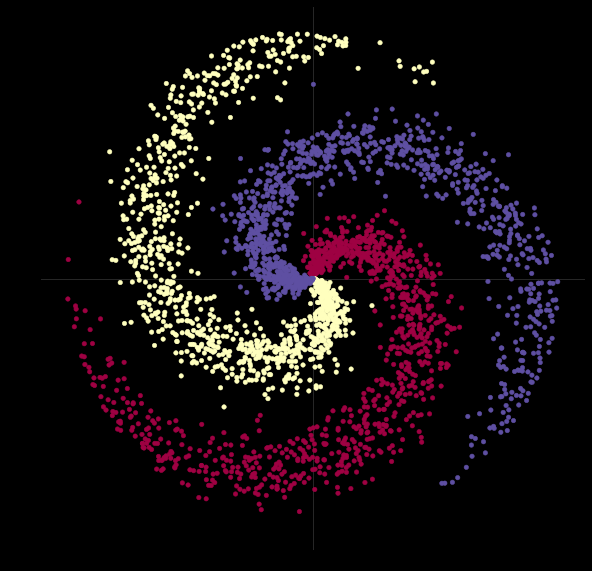
\includegraphics[width=0.5\linewidth]{lectures/03-a/images/data_noise.png} 
\end{center}


\section{Linear Model}
% Authors: Fekade Brook, Nicholas Greenquist, Aaron Wong
% Lecture date: 2/11/2019

Now, let's create a simple neural network with only linear layers.

\begin{minted}{python}
learning_rate = 1e-3
lambda_l2 = 1e-5

device = torch.device("cuda:0" if torch.cuda.is_available() else "cpu")

# nn package to create our linear model
# each Linear module has a weight and bias
model = nn.Sequential(
    nn.Linear(D, H),
    nn.Linear(H, C)
)
model.to(device) #Convert to CUDA

# nn package also has different loss functions.
# we use cross entropy loss for our classification task
criterion = torch.nn.CrossEntropyLoss()

# we use the optim package to apply
# stochastic gradient descent for our parameter updates
# built-in L2
optimizer = torch.optim.SGD(model.parameters(), lr=learning_rate, weight_decay=lambda_l2)

# Training
for t in range(1000):
    
    # Feed forward to get the logits
    y_pred = model(X)
    
    # Compute the loss and accuracy
    loss = criterion(y_pred, y)
    score, predicted = torch.max(y_pred, 1)
    acc = (y == predicted).sum().float() / len(y)
    print("[EPOCH]: %i, [LOSS]: %.6f, [ACCURACY]: %.3f" % (t, loss.item(), acc))
    display.clear_output(wait=True)
    
    # zero the gradients before running
    # the backward pass.
    optimizer.zero_grad()
    
    # Backward pass to compute the gradient
    # of loss w.r.t our learnable params. 
    loss.backward()
    
    # Update params
    optimizer.step()
\end{minted}

First, we set up some hyper parameters and then move the model to the GPU's memory if PyToch detects a GPU. 
This model will move our data from D dimensions to H dimensions, and then back to C. 

As you can see, this model uses CrossEntropyLoss to judge the performance of the classifier. 
It also uses SGD as the optimizer. 
Remember, we prefer stochastic gradient descent over batch gradient descent because most data has a lot of redundancy and we do not need to use every data point to compute the gradient. 

\textbf{epoch}: One full pass through the entire training data. 
We will sweep over every training example here 1000 times. 
That is, we will be running 1000 epochs.

Why do we have to zero the gradients before the backward pass? 
PyTorch automatically accumulates the gradients as it goes through the network. 
If we don't zero out the gradients, we keep adding new gradients to dirty memory which we don't want. 
We want to create a fresh new gradient before each step. 

Why do we add gradients to begin with? 
If we keep adding gradients, we end up with the average gradient over all the training data which is what we would end up with anyways with batch gradient descent.

\textbf{NB}: Always remember to zero your gradients! This is easily forgotten. 

What happens if we invert these two lines ? 

\begin{minted}{python}
optimizer.zero_grad()
loss.backward()
\end{minted}

We'd get nothing as the gradient would always be zero so our model would take no steps. 

What is optimizer.step()? 
This line uses the gradient to find the best direction to change the parameter weights. 
It finds the best direction and takes a ``step'' in that direction to values that give better loss. 

After running this model, we get the following decision boundaries, visualized here:

\begin{center}
	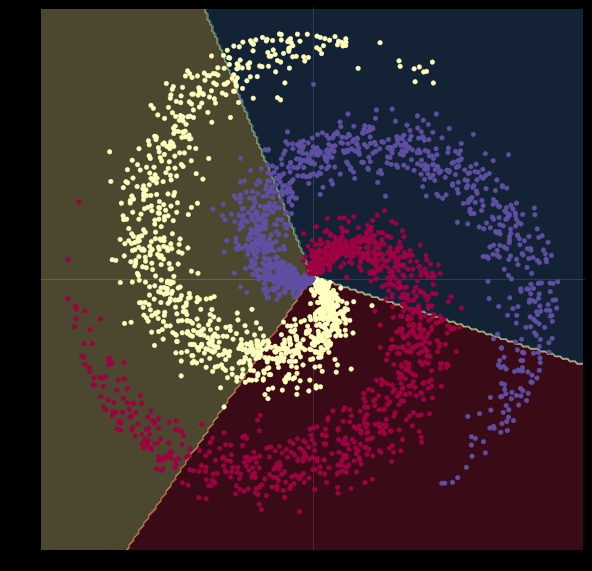
\includegraphics[width=0.5\linewidth]{lectures/03-a/images/linear.png}
\end{center}

What's wrong with this model? 
It's only giving about 50\% accuracy!

Remember, with 3 classes, random guessing would give us 33.33\% accuracy so we are still doing somewhat better than chance. 
This is because the model can do some work by simply rotating the decision boundaries. 

\textbf{NB}: Always print the initial loss before any optimizer steps. 
This is because we need to see if our model is actually improving at all from a random initialization of weights. 

Here is how to compute the initial loss for the model we have above. With three classes, we can compute what our initial loss would be by using
\begin{minted}{python}
-math.log(1/3) # 1/3 because of random guess for 3 classes
# or you can equivalently use:
math.log(3) # outputs 1.09861228867
\end{minted}

This value is what we would see with using a random guess for one of each classes. As we saw from running the notebook, with a Linear Model, we can achieve a final loss of 0.861541 which is lower than initial loss of 1.0986. Computing what the initial loss would have been with random guess and putting that into the loss function is very important because it allows us to see that after some training, we did in fact do 'better.'

\section{Non-Linear Model}
% Authors: Fekade Brook, Nicholas Greenquist, Aaron Wong
% Lecture date: 2/11/2019

Now, let's add a ReLu in between the two linear layers and see what we get.
\begin{minted}{python}
learning_rate = 1e-3
lambda_l2 = 1e-5

model = nn.Sequential(
    nn.Linear(D, H),
    nn.ReLU(),
    nn.Linear(H, C)
)
model.to(device)

# nn package also has different loss functions.
# we use cross entropy loss for our classification task
criterion = torch.nn.CrossEntropyLoss()

# we use the optim package to apply
# ADAM for our parameter updates
# built-in L2
optimizer = torch.optim.Adam(model.parameters(), lr=learning_rate, weight_decay=lambda_l2)

# e = 1.  # plotting purpose

# Training
for t in range(1000):
    
    # Feed forward to get the logits
    y_pred = model(X)
    
    # Compute the loss and accuracy
    loss = criterion(y_pred, y)
    score, predicted = torch.max(y_pred, 1)
    acc = (y == predicted).sum().float() / len(y)
    print("[EPOCH]: %i, [LOSS]: %.6f, [ACCURACY]: %.3f" % (t, loss.item(), acc))
    display.clear_output(wait=True)
    
    # zero the gradients before running
    # the backward pass.
    optimizer.zero_grad()
    
    # Backward pass to compute the gradient
    # of loss w.r.t our learnable params. 
    loss.backward()
    
    # Update params
    optimizer.step()
\end{minted}

WOW: after running this, we get a model that classifies with 0.934 accuracy. 

How does it look? 
Very pretty as you can see for yourselves below: 

\begin{center}
	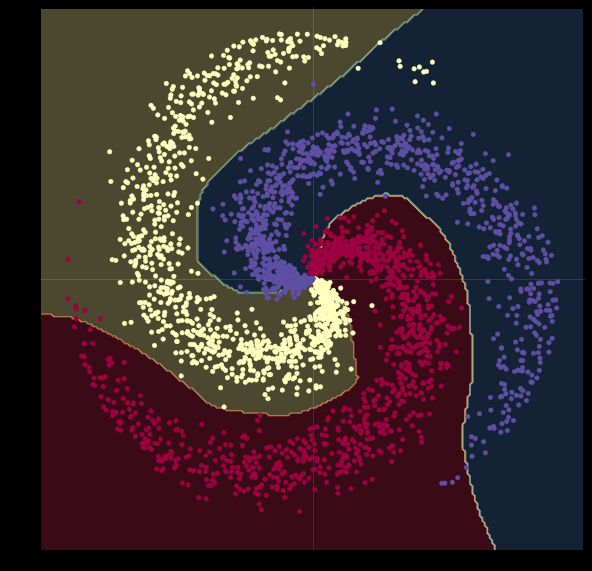
\includegraphics[width=0.5\linewidth]{lectures/03-a/images/relu.png}
\end{center}

Where are we looking from in these visualizations? 
From the bottom up! 
This is because the shape of the data we see here is before any transformations are done on it. 

\section{Skinny Model}
% Authors: Fekade Brook, Nicholas Greenquist, Aaron Wong
% Lecture date: 2/11/2019

Now, let's remove the noise of same input data. 
Let's use a neural network that doesn't expand the input to 100 dimensions this time and see what kind of classifier we get. 

\begin{figure}
	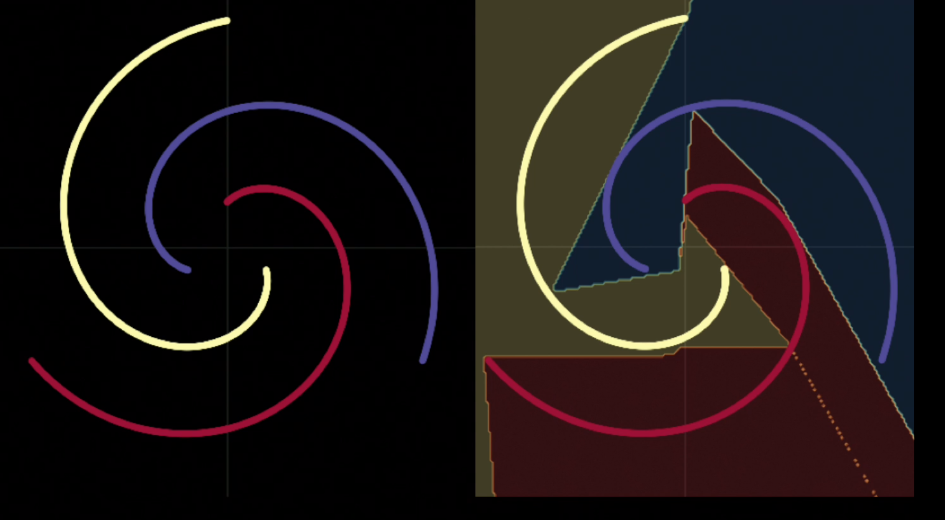
\includegraphics[width=0.85\linewidth]{lectures/03-a/images/not_wide.png}
	\caption{No projection to a higher dimension}
	\label{fig:ugly_low_dim}
\end{figure}

Here is the code that was used to generate a decision boundary like this:

\begin{minted}{python}
# NN model
def two_layer_network(D_in, D_out, hidden_layers, H):

    modules = list()
    in_d = D_in

    for l in range(hidden_layers):
        modules.append(nn.Linear(in_d, H))
        modules.append(nn.LeakyReLU())
        in_d = H
    modules.append(nn.Linear(H, H))  # added layer
    modules.append(nn.Linear(H, D_out))
    return nn.Sequential(*modules)

learning_rate = 1e-2
lambda_l2 = 1e-9

# D = 2, C = 3
model = two_layer_network(D, C, 4, D)
 
# ...use the same code as seen above to train this model
\end{minted}

The final decision boundary is very ugly and rigid. 
This is because we did not expand the dimensions of the data. 
This limits how much we can stretch out the plane to then divide the data. 
However, with enough tweaking of the random seed and rerunning the model, even this constrained model can achieve 100\% accuracy on this data as seen from \cref{fig:ugly_low_dim}. 

Let's see the entire dimension space transformed by this network:

\begin{center}
	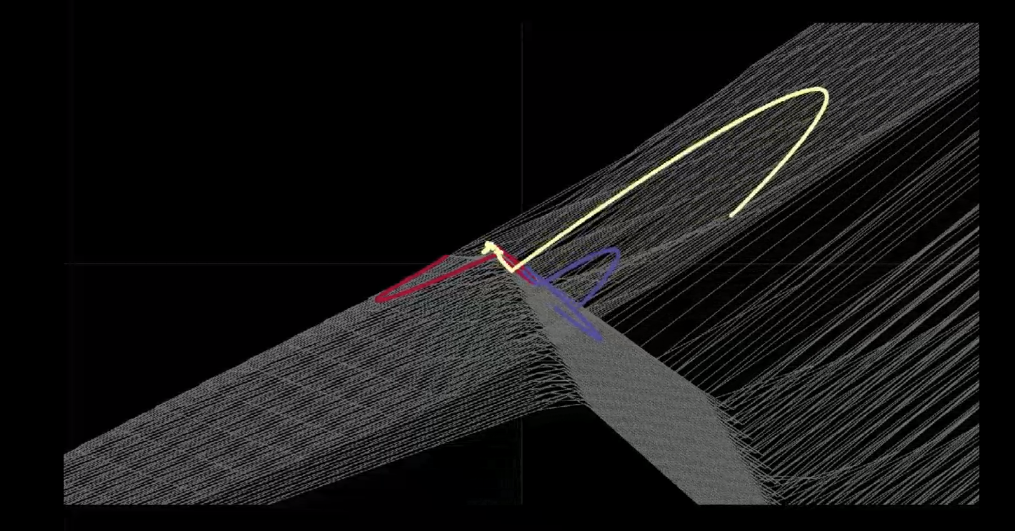
\includegraphics[width=0.85\linewidth]{lectures/03-a/images/stretch.png}
\end{center}

The network actually warps the entire space to make the spirals linearly separable. 

Now, we have seen the decision boundary from the bottom of the network. 
Let's see what the decision boundary looks like from the top of the network:

\begin{center}
	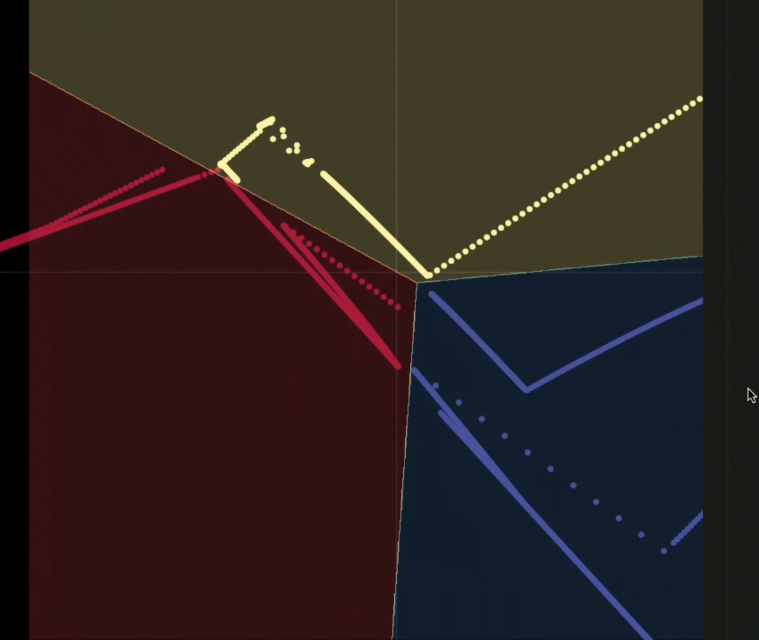
\includegraphics[width=0.5\linewidth]{lectures/03-a/images/top_view_boundary.png}
\end{center}

If you visualize the space after each transformation, you can actually see the ReLu 'cut off' negative points and 'squash' them to 0. 
Here is an example of some of the points 'squashed' by the ReLu after one step:

\begin{center}
	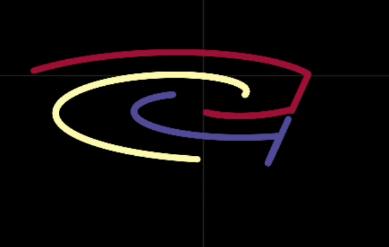
\includegraphics[width=0.85\linewidth]{lectures/03-a/images/squash.png}
\end{center}

In short, the network's job is simply to warp space until we attach a final layer that does a simple classification on the new, easily separated space. 

\noindent\fbox{\begin{minipage}{\textwidth}
\textbf{How do you know this sequence will make this space linearly separable?}
\vspace{1em}

You visually see that the space can be separated by some line. 
They aren't even overlapped so it should be easy given some specific stretching.
\end{minipage}}

One thing to notice is that if you do map to a higher dimension and then back down to the output, you will see smoother decision boundaries. 
The decision boundary we saw with this non-expansive model is more piece-wise.

If you use $\tanh$ or sigmoid non-linearities, the transitions from each new transformed dimension space are much smoother than if you clip and 'squash' with ReLu. 

As Professor LeCun stated, we get these transformations because we are letting the optimizer decide what the next best transformation to run is that minimizes the loss. 

\noindent\fbox{\begin{minipage}{\textwidth}
\textbf{What is bottom up vs top down when discussing networks? }
\vspace{1em}

Input is bottom, output is top (because you climb up hierarchy). 
If you draw the network upside down, it makes an inverted representation.
So, when we say we add classifier on top, it means we add it to the last layer in the network. 
\end{minipage}}

\noindent\fbox{\begin{minipage}{\textwidth}
\textbf{How does ReLu divide the input into subspaces?}
\vspace{1em}

This splitting actually applies to any non-linearity. 
Any time you have one in the activation function, you're basically performing elementary detection. 
So, imagine a threshold function. 
You're basically dividing the input into what section outputs the 1 and what section outputs the -1. 
However, simple threshold functions destroy too much information so we look for softer threshold functions. 
ReLu is an example of a softer threshold that preserves more information. 
\end{minipage}}

In addition to the ReLu, you can also use a Leaky ReLu: 
\href{https://medium.com/tinymind/a-practical-guide-to-relu-b83ca804f1f7}{A Practical Guide to ReLU}

According to Professor LeCun, small networks are good to visualize what is going on but will fail for most problems. 
This spiral problem requires very little width in the network so that's why it works. 

\textbf{NB}: The bigger the network, the easier it is to train as gradient descent has more time to optimize.

In addition to this note, the networks that expand to higher dimensions are trained much better and result in smoother decision boundaries. 
These boundaries are still piece-wise linear if you zoom in enough, but its almost impossible to see it from the output view. 
%%%%%%%%%%%%%%%%%%%%%%%%%%%%%%%%%%%%%%%%%%
\part{Applications}\label{prt:apps}
%%%%%%%%%%%%%%%%%%%%%%%%%%%%%%%%%%%%%%%%%%
%%%%%%%%%%%%%%%%%%%%%%%%%%%%%%%%%%%%%%%%%%
\part{Papers summary}\label{prt:papers}
%%%%%%%%%%%%%%%%%%%%%%%%%%%%%%%%%%%%%%%%%%

The end.  % \part needs to be followed by something.

\end{document}
